\documentclass[journal,twoside,web]{ieeecolor}
\usepackage{generic}
\usepackage{cite}
\usepackage{amsmath,amssymb,amsfonts}
\usepackage{graphicx}
\usepackage{algorithm,algorithmic}
\usepackage{textcomp}
\usepackage{float}
\usepackage{placeins}
\usepackage{url}
\usepackage{hyperref}
\hypersetup{
    colorlinks=true,
    linkcolor=blue,
    filecolor=magenta,
    urlcolor=blue,
}

\usepackage{tikz}
\usepackage{pgfplots}
%\pgfplotsset{compat=1.18}

\def\BibTeX{{\rm B\kern-.05em{\sc i\kern-.025em b}\kern-.08em
    T\kern-.1667em\lower.7ex\hbox{E}\kern-.125emX}}
\markboth{\hfill Universidade Federal de Mato Grosso do Sul}
{Trabalho: Fonte 12~V e 1~A}

\begin{document}
\title{\vspace*{2cm}Trabalho prático - Fonte de tensão 12~V e 1~A}
\author{Luis M. T. Fialho, Thiago P. de Souza, Maykon K. F. Tamanaha, e Ricardo Y. S. da Silva
\thanks{9 de Outubro de 2026}}

\maketitle

% Macro de pendencias (definida apenas se ainda nao existir; requer xcolor, carregado tambem por tikz).
\providecommand{\pendente}[1]{\textcolor{red}{[PENDENTE: #1]}}

{
\small\sffamily\selectfont
\textbf{\textit{Resumo} --- Este trabalho apresenta o projeto, a montagem em \textit{protoboard} e a verificação experimental de uma fonte linear regulada de $12\,\text{V}$ DC, projetada para corrente nominal de $1\,\text{A}$. O circuito emprega transformador de $12\,\text{V}+12\,\text{V}$ com derivação central, retificador de onda completa com dois diodos 1N4007, capacitor eletrolítico de $4700\,\mu\text{F} / 25\,\text{V}$, regulador LM7812 e dois capacitores de $100\,\text{nF}$, além de chave e fusíveis de proteção. Os ensaios com multímetro e osciloscópio percorreram os estágios da fonte: secundário do transformador com pico de $19{,}1\,\text{V}$ em vazio, onda retificada pulsante de $120\,\text{Hz}$, tensão filtrada de $17{,}96\,\text{V}$ com \textit{ripple} em dente de serra e saída regulada de $11{,}95\,\text{V}$, desvio de $-0{,}42\%$ em relação a $12\,\text{V}$. A corrente de $0{,}12\,\text{A}$ sobre um resistor de $100\,\Omega$ é compatível com a lei de Ohm. A fonte foi validada experimentalmente até $0{,}12\,\text{A}$; a operação em $1\,\text{A}$ foi apenas analisada teoricamente. A amplitude absoluta do \textit{ripple} não pôde ser validada, pois o fator da ponta do osciloscópio não foi registrado. O multímetro foi usado na função DC no Experimento~1, e o Experimento~5 não discriminou variação de carga. Recomendam-se dissipador no regulador, fusível de retardo e ensaio a $1\,\text{A}$.}

\textbf{\textit{Palavras-chave} --- Capacitor eletrolítico, chave liga/desliga, derivação central, filtro capacitivo, fonte de alimentação linear, fusível, LM7812, retificador de onda completa, transformador.}
}

\vspace{1em}

\begin{abstract}
This paper presents the design, breadboard assembly, and experimental verification of a $12\,\text{V}$ DC linear regulated power supply rated for a nominal current of $1\,\text{A}$. The circuit uses a $12\,\text{V}+12\,\text{V}$ center-tapped transformer, a full-wave rectifier with two 1N4007 diodes, a $4700\,\mu\text{F} / 25\,\text{V}$ electrolytic capacitor, an LM7812 regulator, and two $100\,\text{nF}$ capacitors, together with a switch and protection fuses. Multimeter and oscilloscope tests covered the stages of the supply: a transformer secondary with a no-load peak of $19.1\,\text{V}$, a pulsating full-wave rectified waveform of $120\,\text{Hz}$, a filtered voltage of $17.96\,\text{V}$ with sawtooth ripple, and a regulated output of $11.95\,\text{V}$, a deviation of $-0.42\%$ from $12\,\text{V}$. The current of $0.12\,\text{A}$ through a $100\,\Omega$ resistor is consistent with Ohm's law. The supply was experimentally validated up to $0.12\,\text{A}$; operation at $1\,\text{A}$ was only analyzed theoretically. The absolute ripple amplitude could not be validated because the oscilloscope probe factor was not recorded. The multimeter was used in its DC function in Experiment~1, and Experiment~5 could not discriminate load variation. A heat sink for the regulator, a slow-blow fuse, and a test at $1\,\text{A}$ are recommended.
\end{abstract}

\begin{IEEEkeywords}
Capacitive filter, center tap, electrolytic capacitor, full-wave rectifier, fuse, linear power supply, LM7812, ON/OFF switch, transformer.
\end{IEEEkeywords}


\section{Introdução}

\IEEEPARstart{A}{s} fontes de alimentação lineares desempenham um papel fundamental na eletrônica analógica e digital, sendo responsáveis por converter a tensão alternada (AC) proveniente da rede elétrica comercial em uma tensão contínua (DC) estável e regulada, adequada para alimentar circuitos eletrônicos sensíveis. Em aplicações laboratoriais e de bancada, a estabilidade do nível DC de saída, a imunidade a variações da rede elétrica e a minimização da ondulação residual (\textit{ripple}) são parâmetros críticos para garantir a integridade dos sinais e a confiabilidade dos dispositivos alimentados.

Este relatório descreve o projeto, o dimensionamento teórico, a implementação em \textit{protoboard} e a verificação experimental de uma fonte de alimentação linear regulada de $12\,\text{V}$ DC com capacidade nominal de até $1\,\text{A}$, desenvolvida como Trabalho Prático da disciplina de Circuitos Eletrônicos na Faculdade de Computação (FACOM) da Universidade Federal de Mato Grosso do Sul (UFMS). Ao longo das seções seguintes, detalham-se o embasamento teórico de cada bloco funcional, a arquitetura montada em laboratório com levantamento de componentes e custos, bem como a análise quantitativa das formas de onda e grandezas medidas em seis ensaios experimentais progressivos.

\subsection{Princípio de Funcionamento e Dimensionamento Teórico}

O funcionamento de uma fonte de alimentação linear regulada baseia-se em quatro estágios principais encadeados --- transformação, retificação, filtragem e regulação --- complementados por dispositivos de acionamento e proteção elétrica.

\subsubsection{Estágio de Transformação}
O primeiro estágio utiliza um transformador abaixador com tomada central (\textit{center-tap}), descrito como ``$12\,\text{V}+12\,\text{V}$, $1\,\text{A}$''. O enrolamento primário bivolt ($127\,\text{V}/220\,\text{V}$) é conectado à rede elétrica de $127\,\text{V}$ RMS ($60\,\text{Hz}$), e o secundário fornece tensão nominal simétrica de $12\,\text{V} + 12\,\text{V}$ AC com corrente nominal de $1\,\text{A}$, além de garantir isolação galvânica em relação à rede. A potência aparente (VA) do transformador não foi informada e, por isso, não é utilizada neste relatório. Para uma forma de onda senoidal ideal de valor eficaz $V_{\text{RMS}}$, a amplitude de pico $V_p$ é dada por:
\begin{equation}
V_p = V_{\text{RMS}}\sqrt{2}.
\label{eq:vpico}
\end{equation}
Para o valor nominal de $12\,\text{V}$ RMS, obtém-se $V_p \approx 16{,}97\,\text{V}$. Transformadores de baixa potência costumam apresentar tensão em vazio superior à nominal; neste trabalho, a tensão em vazio foi obtida por medição (Seção~\ref{sec:analise}, Experimento~1).

\subsubsection{Estágio de Retificação}
A tensão alternada do secundário é aplicada a um retificador de onda completa com derivação central composto por dois diodos de silício 1N4007. Com o fio central aterrado como referência de $0\,\text{V}$ (GND), cada diodo conduz em um dos semiciclos da rede, direcionando ambos os semiciclos com polaridade positiva para a carga. Em comparação à ponte retificadora de quatro diodos, essa topologia provoca a queda de apenas uma junção PN ($V_D \approx 0{,}7\,\text{V}$) por semiciclo:
\begin{equation}
V_{p,\text{ret}} = V_p - V_D.
\label{eq:vpret}
\end{equation}
Como ambos os semiciclos são aproveitados, a frequência da tensão pulsante dobra em relação à rede elétrica ($f_{\text{ret}} = 2f_{\text{rede}} = 120\,\text{Hz}$, período $T_{\text{ret}} = 8{,}33\,\text{ms}$). Sem filtro capacitivo, o valor médio (DC) dessa onda retificada ideal de pico $V_{p,\text{ret}}$ é:
\begin{equation}
V_{\text{DC,sem filtro}} = \frac{2 V_{p,\text{ret}}}{\pi}.
\label{eq:vdc_sem_filtro}
\end{equation}
Nessa topologia, o diodo em corte fica sujeito a uma tensão reversa de cerca de duas vezes o pico do secundário. Com o pico em vazio medido de $19{,}1\,\text{V}$, a tensão reversa de pico (PIV) estimada é $\text{PIV} \approx 2V_p \approx 38\,\text{V}$, muito abaixo da tensão reversa repetitiva máxima de $1000\,\text{V}$ do 1N4007 (\textit{datasheet}~\cite{ds_1n4007}).

\subsubsection{Estágio de Filtragem Capacitiva}
Para converter a tensão pulsante em um nível contínuo elevado, conecta-se em paralelo à saída dos diodos um capacitor eletrolítico de alta capacitância ($C = 4700\,\mu\text{F} / 25\,\text{V}$). O capacitor carrega-se rapidamente próximo ao pico $V_{p,\text{ret}}$ e mantém a alimentação do circuito enquanto os diodos permanecem reversamente polarizados, descarregando-se até o pico seguinte. A ondulação residual pico a pico resultante (\textit{ripple}, $\Delta V_r$) pode ser estimada em primeira aproximação pela descarga linear sob corrente constante $I_{\text{carga}}$:
\begin{equation}
\Delta V_r \approx \frac{I_{\text{carga}}}{f_{\text{ret}}\, C}.
\label{eq:ripple}
\end{equation}
Para a condição de projeto ($I_{\text{carga}} = 1\,\text{A}$, $f_{\text{ret}} = 120\,\text{Hz}$ e $C = 4700\,\mu\text{F}$), obtém-se $\Delta V_r \approx 1{,}77\,\text{V}_{\text{pp}}$. A verificação dos vales da tensão filtrada nessa condição, inclusive com redução de $10\%$ na rede, é apresentada na análise teórica da Seção~\ref{sec:teoria1A}.

O valor de $25\,\text{V}$ do capacitor corresponde à sua tensão nominal de trabalho. A margem em relação a esse valor é avaliada com o pico em vazio medido de $19{,}1\,\text{V}$; com sobretensão de $+10\%$ na rede, o pico seria de $\approx 21\,\text{V}$ (cálculo), abaixo de $25\,\text{V}$.

\subsubsection{Estágio de Regulação e Desacoplamento}
A estabilização final é realizada pelo circuito integrado regulador linear de tensão positiva LM7812 (encapsulamento TO-220), cuja saída é de $12\,\text{V}$ DC com tolerância de $\pm 4\%$ ($11{,}5\,\text{V}$ a $12{,}5\,\text{V}$), conforme \href{https://www.ti.com/lit/ds/symlink/lm340.pdf}{Datasheet do LM7812} (Texas Instruments, documento \texttt{SNOSBT0L}), com proteção térmica e limitação de corrente internas. O componente físico utilizado na montagem possui gravação comercial \texttt{SCE7812} (lote genérico/remarcado sem folha de dados própria publicada pelo fabricante ou distribuidor), adotando-se o \textit{datasheet} da Texas Instruments como referência técnica; o valor da corrente de limitação não é citado neste relatório por não ter sido confirmado em \textit{datasheet} do fabricante utilizado. Para assegurar a regulação, a tensão mínima de entrada no pino~1 não deve cair abaixo da soma da tensão de saída com a tensão de \textit{dropout} do CI ($\approx 2\,\text{V}$), exigindo $V_{\text{in}} \gtrsim 14\,\text{V}$. Junto ao regulador são instalados dois capacitores cerâmicos de $100\,\text{nF}$: o da entrada (pino~1 ao GND) contribui para a estabilidade do regulador, e o da saída (pino~3 ao GND) atenua ruído de alta frequência. Esses capacitores não são o elemento responsável pela rejeição da ondulação de $120\,\text{Hz}$.

\subsubsection{Dispositivos de Acionamento e Proteção}
O circuito inclui no lado primário uma chave gangorra liga/desliga (SPST) em série com um fusível de $500\,\text{mA}$, instalado entre o plugue da tomada e o interruptor. No lado secundário, entre o nó comum dos catodos dos diodos retificadores e o restante do circuito, foi inserido um fusível de $1{,}5\,\text{A}$.

O fusível de $500\,\text{mA}$ protege o primário. O de $1{,}5\,\text{A}$ possui valor acima da corrente nominal de $1\,\text{A}$ e foi adotado para suportar a corrente de carga do capacitor de $4700\,\mu\text{F}$ na energização, sem atuar indevidamente. Esse fusível não interrompe sobrecargas contínuas entre $1\,\text{A}$ e $1{,}5\,\text{A}$; sua função é principalmente a proteção contra curto-circuito. O regulador possui limitação interna de corrente, cujo valor depende do \textit{datasheet} do fabricante utilizado. O tipo e a tensão nominal dos fusíveis não foram especificados pelo vendedor. Como melhoria, recomenda-se fusível de retardo, com tensão nominal de $250\,\text{V}$ CA, no primário.

\subsection{Critérios de Aceitação}

Para a avaliação dos resultados, adotam-se os seguintes critérios:
\begin{enumerate}
    \item tensão de saída de $12\,\text{V} \pm 4\%$ ($11{,}5\,\text{V}$ a $12{,}5\,\text{V}$), faixa do \textit{datasheet} do regulador~\cite{ds_lm7812};
    \item \textit{ripple} na saída muito menor que na entrada do regulador;
    \item capacidade nominal de corrente de $1\,\text{A}$ (especificação do trabalho).
\end{enumerate}
A especificação do trabalho não define tolerâncias numéricas. A faixa de $\pm 4\%$ é a do \textit{datasheet} do regulador, e os demais critérios são qualitativos.


\section{Procedimento Experimental}

\subsection{Local, Arquitetura e Lógica de Montagem}

A montagem e a verificação experimental foram realizadas em \textit{protoboard} de $830$ pontos nas bancadas do Laboratório de Redes e Eletrônica da FACOM/UFMS. A montagem seguiu o encadeamento dos estágios de conversão de energia, o que permitiu testar cada bloco antes de integrar a carga final. O diagrama completo do circuito é apresentado na Figura~\ref{fig:esquematico}, e os pontos de medição dos experimentos estão indicados por E1 a E6. O regulador LM7812 foi utilizado sem dissipador de calor.

\begin{figure*}[t]
\centering
\resizebox{0.96\textwidth}{!}{%
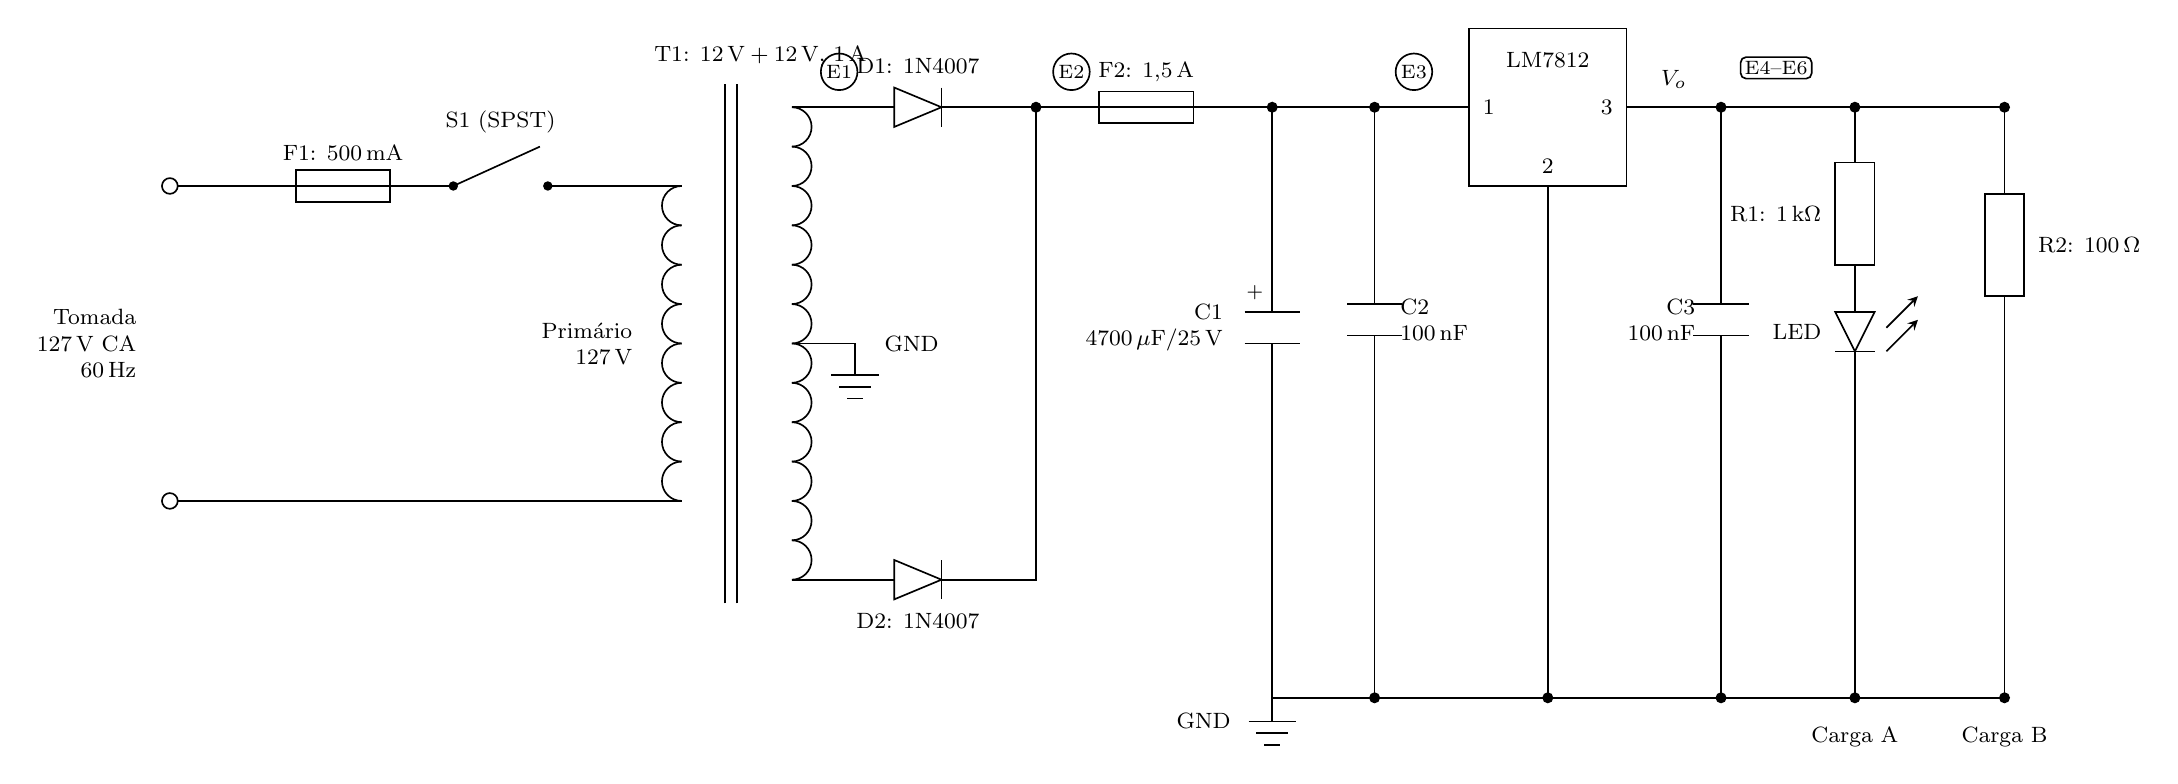
\begin{tikzpicture}[line width=0.6pt,>=stealth,font=\footnotesize]
% --- Tomada, F1 e chave S1 (primario)
\draw (0,5) circle (0.1);
\draw (0,1) circle (0.1);
\node[anchor=east,align=right] at (-0.3,3) {Tomada\\$127\,\text{V}$ CA\\$60\,\text{Hz}$};
\draw (0.1,5)--(1.6,5);
\draw (0.1,1)--(6.5,1);
\draw (1.6,4.8) rectangle (2.8,5.2);
\draw (1.6,5)--(2.8,5);
\node[above] at (2.2,5.2) {F1: $500\,\text{mA}$};
\draw (2.8,5)--(3.6,5);
\fill (3.6,5) circle (0.06);
\fill (4.8,5) circle (0.06);
\draw (3.6,5)--(4.7,5.5);
\draw (4.8,5)--(6.5,5);
\node[above] at (4.2,5.55) {S1 (SPST)};
% --- Transformador T1 (primario, nucleo, secundario com derivacao central)
\foreach \i in {0,...,7} {\draw (6.5,{5-\i*0.5}) arc (90:270:0.25);}
\node[anchor=east,align=right] at (6.0,3) {Primário\\$127\,\text{V}$};
\draw (7.05,-0.3)--(7.05,6.3);
\draw (7.2,-0.3)--(7.2,6.3);
\foreach \i in {0,...,11} {\draw (7.9,{6-\i*0.5}) arc (90:-90:0.25);}
\node[above,align=center] at (7.5,6.4) {T1: $12\,\text{V}+12\,\text{V}$, $1\,\text{A}$};
% derivacao central (GND)
\draw (7.9,3)--(8.7,3);
\draw (8.7,3)--(8.7,2.6);
\draw (8.4,2.6)--(9.0,2.6);
\draw (8.5,2.45)--(8.9,2.45);
\draw (8.6,2.3)--(8.8,2.3);
\node[right] at (8.95,3) {GND};
% --- Diodos D1 e D2
\draw (7.9,6)--(9.2,6);
\draw[fill=white] (9.2,6.25)--(9.2,5.75)--(9.8,6)--cycle;
\draw (9.8,6.25)--(9.8,5.75);
\draw (9.8,6)--(11,6);
\node[above] at (9.5,6.3) {D1: 1N4007};
\draw (7.9,0)--(9.2,0);
\draw[fill=white] (9.2,0.25)--(9.2,-0.25)--(9.8,0)--cycle;
\draw (9.8,0.25)--(9.8,-0.25);
\draw (9.8,0)--(11,0)--(11,6);
\node[below] at (9.5,-0.3) {D2: 1N4007};
\fill (11,6) circle (0.07);
% --- Fusivel F2, capacitor C1 e trilho nao regulado
\draw (11,6)--(11.8,6);
\draw (11.8,5.8) rectangle (13,6.2);
\draw (11.8,6)--(13,6);
\node[above] at (12.4,6.2) {F2: $1{,}5\,\text{A}$};
\draw (13,6)--(16.5,6);
\fill (14,6) circle (0.07);
\draw (14,6)--(14,3.4);
\draw (13.65,3.4)--(14.35,3.4);
\draw (13.65,3.0)--(14.35,3.0);
\draw (14,3.0)--(14,-1.5);
\node at (13.78,3.65) {\scriptsize $+$};
\node[left,align=right] at (13.5,3.2) {C1\\$4700\,\mu\text{F}/25\,\text{V}$};
% --- Capacitor C2 (entrada do regulador)
\fill (15.3,6) circle (0.07);
\draw (15.3,6)--(15.3,3.5);
\draw (14.95,3.5)--(15.65,3.5);
\draw (14.95,3.1)--(15.65,3.1);
\draw (15.3,3.1)--(15.3,-1.5);
\fill (15.3,-1.5) circle (0.07);
\node[right,align=left] at (15.5,3.3) {C2\\$100\,\text{nF}$};
% --- Regulador LM7812
\draw (16.5,5) rectangle (18.5,7);
\node at (17.5,6.6) {LM7812};
\node at (16.75,6.0) {1};
\node at (18.25,6.0) {3};
\node at (17.5,5.25) {2};
\draw (17.5,5)--(17.5,-1.5);
\fill (17.5,-1.5) circle (0.07);
% --- Saida, capacitor C3 e cargas
\draw (18.5,6)--(23.3,6);
\fill (19.7,6) circle (0.07);
\draw (19.7,6)--(19.7,3.5);
\draw (19.35,3.5)--(20.05,3.5);
\draw (19.35,3.1)--(20.05,3.1);
\draw (19.7,3.1)--(19.7,-1.5);
\fill (19.7,-1.5) circle (0.07);
\node[left,align=right] at (19.5,3.3) {C3\\$100\,\text{nF}$};
\node at (19.1,6.35) {$V_o$};
% carga A: R1 + LED
\fill (21.4,6) circle (0.07);
\draw (21.4,6)--(21.4,5.3);
\draw (21.15,4.0) rectangle (21.65,5.3);
\draw (21.4,4.0)--(21.4,3.4);
\draw[fill=white] (21.15,3.4)--(21.65,3.4)--(21.4,2.9)--cycle;
\draw (21.15,2.9)--(21.65,2.9);
\draw (21.4,2.9)--(21.4,-1.5);
\fill (21.4,-1.5) circle (0.07);
\draw[->] (21.8,3.2)--(22.2,3.6);
\draw[->] (21.8,2.9)--(22.2,3.3);
\node[left] at (21.1,4.65) {R1: $1\,\text{k}\Omega$};
\node[left] at (21.1,3.15) {LED};
\node at (21.4,-2.0) {Carga A};
% carga B: R2
\fill (23.3,6) circle (0.07);
\draw (23.3,6)--(23.3,4.9);
\draw (23.05,3.6) rectangle (23.55,4.9);
\draw (23.3,3.6)--(23.3,-1.5);
\fill (23.3,-1.5) circle (0.07);
\node[right] at (23.6,4.25) {R2: $100\,\Omega$};
\node at (23.3,-2.0) {Carga B};
% --- Trilho de GND
\draw (14,-1.5)--(23.3,-1.5);
\draw (14,-1.5)--(14,-1.8);
\draw (13.7,-1.8)--(14.3,-1.8);
\draw (13.8,-1.95)--(14.2,-1.95);
\draw (13.9,-2.1)--(14.1,-2.1);
\node[left] at (13.6,-1.8) {GND};
% --- Marcadores de medicao
\node[draw,circle,inner sep=1pt,font=\scriptsize] at (8.5,6.45) {E1};
\node[draw,circle,inner sep=1pt,font=\scriptsize] at (11.45,6.45) {E2};
\node[draw,circle,inner sep=1pt,font=\scriptsize] at (15.8,6.45) {E3};
\node[draw,rounded corners=2pt,inner sep=1.5pt,font=\scriptsize] at (20.4,6.5) {E4--E6};
\end{tikzpicture}}
\caption{Diagrama esquemático da fonte de $12\,\text{V}$: tomada de $127\,\text{V}$, fusível F1 ($500\,\text{mA}$), chave S1, transformador T1 com derivação central (GND), diodos D1 e D2 (1N4007), fusível F2 ($1{,}5\,\text{A}$), capacitor C1 ($4700\,\mu\text{F}/25\,\text{V}$), regulador LM7812 (pinos 1, 2 e 3), capacitores C2 e C3 ($100\,\text{nF}$) e as cargas de ensaio (R1 + LED e R2). Em E2, o capacitor C1 foi removido e um resistor de $1\,\text{k}\Omega$ foi conectado ao GND na etapa sem filtro.}
\label{fig:esquematico}
\end{figure*}

\begin{enumerate}
    \item \textbf{Entrada AC e proteção primária:} O plugue conectado à rede elétrica de $127\,\text{V}$ passa por um porta-fusível volante com fusível de $500\,\text{mA}$ e segue para uma chave gangorra liga/desliga (SPST), que alimenta o enrolamento primário do transformador ($12\,\text{V}+12\,\text{V}$, $1\,\text{A}$).
    \item \textbf{Secundário e retificação:} O fio preto da derivação central do secundário foi ligado ao barramento de referência (GND) da \textit{protoboard}. Os dois fios vermelhos das extremidades do secundário foram conectados aos anodos de dois diodos 1N4007, cujos catodos foram interligados em um mesmo nó.
    \item \textbf{Proteção secundária e filtragem:} Do nó comum dos catodos, um fio conduz o sinal retificado por um segundo porta-fusível volante, com o fusível de $1{,}5\,\text{A}$, até o barramento positivo da \textit{protoboard} (nó de tensão não regulada). Sobre esse nó ligam-se em paralelo o capacitor eletrolítico de $4700\,\mu\text{F} / 25\,\text{V}$ (terminal positivo na linha retificada e negativo no GND), o primeiro capacitor de $100\,\text{nF}$ e o pino~1 (entrada) do LM7812.
    \item \textbf{Regulação e saída:} O pino~2 (GND) do LM7812 conecta-se ao barramento de referência. O pino~3 (saída regulada de $12\,\text{V}$) liga-se ao segundo capacitor de $100\,\text{nF}$, em paralelo com o GND, e aos pontos de conexão das cargas de ensaio (LED em série com resistor de $1\,\text{k}\Omega$, e resistor de $100\,\Omega$).
\end{enumerate}

\textbf{Segurança.} O primário do transformador é alimentado pela rede por meio do plugue, de um fusível e de uma chave, e o transformador permaneceu fora da \textit{protoboard}, de modo que apenas o secundário de baixa tensão foi levado à \textit{protoboard}. Recomenda-se desligar a montagem da tomada antes de remover ou inserir componentes, como foi feito na troca do capacitor e do resistor no Experimento~2, e manter isoladas as conexões do lado da rede.

\subsection{Materiais Utilizados e Custos}

Para os ensaios foram empregados um multímetro digital Victor~88B (Skill-Tec) e um osciloscópio digital Gratten GA1102CAL ($100\,\text{MHz}$, $1\,\text{GSa/s}$). A Tabela~\ref{tab:bom} relaciona os componentes e acessórios adquiridos e utilizados na construção da fonte e nos testes.

\begin{table}[H]
\caption{Lista de componentes utilizados na montagem e custos em reais.}
\label{tab:bom}
\centering
\scriptsize
\setlength{\tabcolsep}{3pt}
\begin{tabular}{cp{6.5cm}}
\hline
Qtd. & Componente / Especificação \\
\hline
1 & Transformador $127/220\,\text{V} \to 12+12\,\text{V}$ ($1\,\text{A}$) \\
1 & Regulador de tensão LM7812 ($12\,\text{V}$, TO-220) \\
1 & Capacitor eletrolítico $4700\,\mu\text{F} / 25\,\text{V}$ \\
2 & Capacitores $100\,\text{nF}$ (104) \\
2 & Diodos retificadores 1N4007 \\
2 & Porta-fusíveis \textit{inline} + fusíveis ($500\,\text{mA}$ e $1{,}5\,\text{A}$); tipo e tensão nominal não especificados pelo vendedor \\
1 & Chave gangorra liga/desliga (SPST) \\
1 & Plugue macho 2P padrão NBR 14136 ($10\,\text{A}$) \\
1 & \textit{Protoboard} $830$ pontos \\
1 & Kit LED $5\,\text{mm}$, resistores ($1\,\text{k}\Omega$; $100\,\Omega$) e fios \\
\hline
\textbf{Total:} & \textbf{R\$ 133} \\
\hline
\end{tabular}
\end{table}

\subsection{Metodologia dos Ensaios Experimentais}

A caracterização da fonte foi conduzida em seis experimentos sequenciais, da saída alternada do transformador até a regulação de carga e a corrente na saída final. Nas capturas do osciloscópio, o fator de atenuação configurado no canal e a posição da chave da ponta nem sempre coincidiram; por isso, os resultados são apresentados como valor exibido, fator aplicado e valor real (Seção~\ref{sec:analise}).

\begin{enumerate}
    \item \textbf{Experimento 1 --- Saída do transformador (pré-retificação):} Sem carga na saída de $12\,\text{V}$, a referência (garra) foi posicionada no fio preto central (GND) e a ponta de medição em um dos terminais vermelhos do secundário, antes dos diodos. O osciloscópio foi utilizado em acoplamento DC. O multímetro permaneceu na escala de $20\,\text{V}$ DC, e não em V$\sim$ (tensão alternada); trata-se de um erro de procedimento, e a leitura obtida não é resultado válido do ensaio.
    \item \textbf{Experimento 2 --- Onda pós-diodos (sem e com filtro capacitivo):} Com a montagem desligada da tomada, o capacitor eletrolítico de $4700\,\mu\text{F}$ foi removido e um resistor de $1\,\text{k}\Omega$ foi inserido entre o nó pós-fusível e o GND. A forma de onda foi registrada no osciloscópio em acoplamento DC. Em seguida, com a montagem novamente desligada, o resistor foi retirado, o capacitor foi reinstalado e a captura foi repetida.
    \item \textbf{Experimento 3 --- Filtro e \textit{ripple} antes do LM7812 (pino 1):} A tensão DC no pino~1 foi medida com o multímetro (escala $20\,\text{V}$ DC). Em seguida, o osciloscópio em acoplamento AC, com $2{,}00\,\text{mV/div}$, $5{,}00\,\text{ms/div}$, limite de banda (B) e filtro (F) ativos, registrou a ondulação em duas condições: saída de $12\,\text{V}$ em aberto e, depois, com LED em série com resistor de $1\,\text{k}\Omega$ entre o pino~3 e o GND. A posição da chave $1\times$/$10\times$ da ponta não foi registrada.
    \item \textbf{Experimento 4 --- Saída regulada de $12\,\text{V}$ (pino 3):} Com o LED e o resistor de $1\,\text{k}\Omega$ conectados na saída, mediram-se a tensão DC no pino~3 com o multímetro ($20\,\text{V}$ DC) e o sinal residual com o osciloscópio em acoplamento AC ($2{,}00\,\text{mV/div}$, $5{,}00\,\text{ms/div}$, B e F ativos). A posição da chave da ponta também não foi registrada.
    \item \textbf{Experimento 5 --- Regulação de carga:} Com o multímetro na escala de $20\,\text{V}$ DC entre o pino~3 e o GND, compararam-se as leituras sem carga (LED desconectado) e com a carga de ensaio (LED + resistor de $1\,\text{k}\Omega$).
    \item \textbf{Experimento 6 --- Corrente com carga de $100\,\Omega$:} Um resistor de $100\,\Omega$ foi conectado ao GND e o multímetro foi inserido em série entre o pino~3 do LM7812 e o outro terminal do resistor. A ponta vermelha foi conectada ao borne de $20\,\text{A}$ e a ponta preta ao borne COM, e a corrente indicada foi $0{,}12\,\text{A}$. Na fotografia, a posição do seletor não coincide com o borne utilizado, e a resolução da indicação é de $0{,}01\,\text{A}$.
\end{enumerate}


\section{Análise dos Dados}
\label{sec:analise}

Nesta seção apresentam-se as medições obtidas nos seis ensaios, realizadas com o multímetro digital Victor~88B e o osciloscópio digital Gratten~GA1102CAL, confrontadas com as Eqs.~\eqref{eq:vpico} a~\eqref{eq:ripple} e com as especificações dos componentes. Cada informação é classificada como medida (captura ou leitura), calculada (equação mostrada), de \textit{datasheet} (com citação) ou hipótese (rotulada como \textit{hipótese, não verificada}). Para o osciloscópio, informam-se o valor exibido, o fator aplicado e o valor real. O fator de atenuação $10\times$ (fator $1/10$ sobre o valor exibido) dos Experimentos~1 e~2B foi validado pela plausibilidade dos valores e pela leitura de $17{,}96\,\text{V}$ no multímetro; para a amplitude do \textit{ripple} (Experimentos~3 e~4), o fator da ponta não foi registrado e não está validado.

\subsection{Experimento 1 --- Saída do Transformador (Pré-Retificação)}

\textbf{Condição:} secundário em vazio, com a derivação central (fio preto) como referência de $0\,\text{V}$, antes dos diodos. As Figuras~\ref{fig:exp1-proto}, \ref{fig:exp1-multi} e~\ref{fig:exp1-osc} mostram, respectivamente, a montagem, a leitura do multímetro e a captura do osciloscópio.

\begin{figure}[H]
\centering
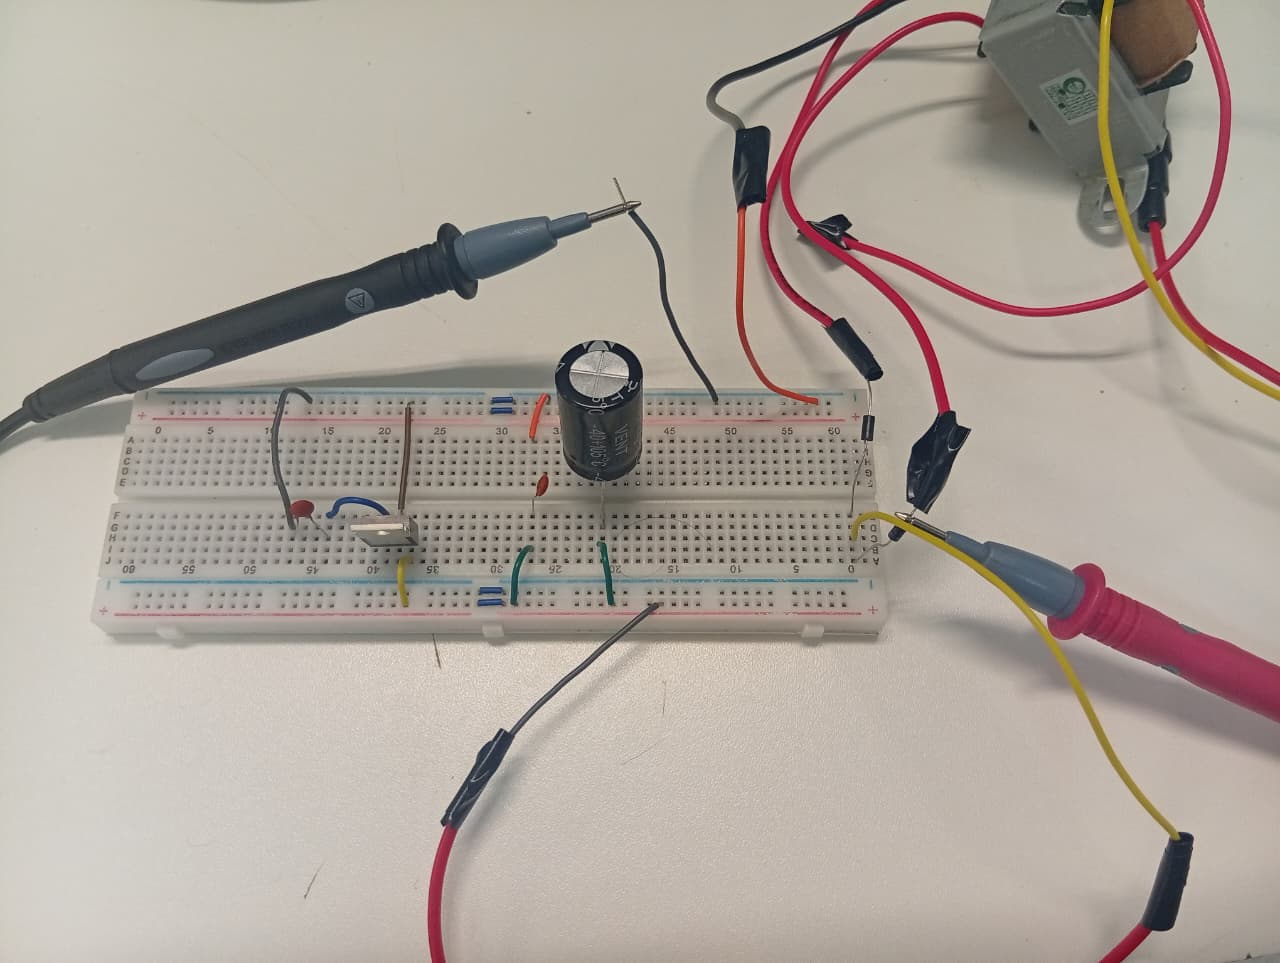
\includegraphics[width=\columnwidth,height=5.6cm,keepaspectratio]{Images/exp1_protoboard-multimetro.jpeg}
\caption{Experimento 1 --- Montagem para medição no secundário do transformador, antes dos diodos.}
\label{fig:exp1-proto}
\end{figure}

\begin{figure}[H]
\centering
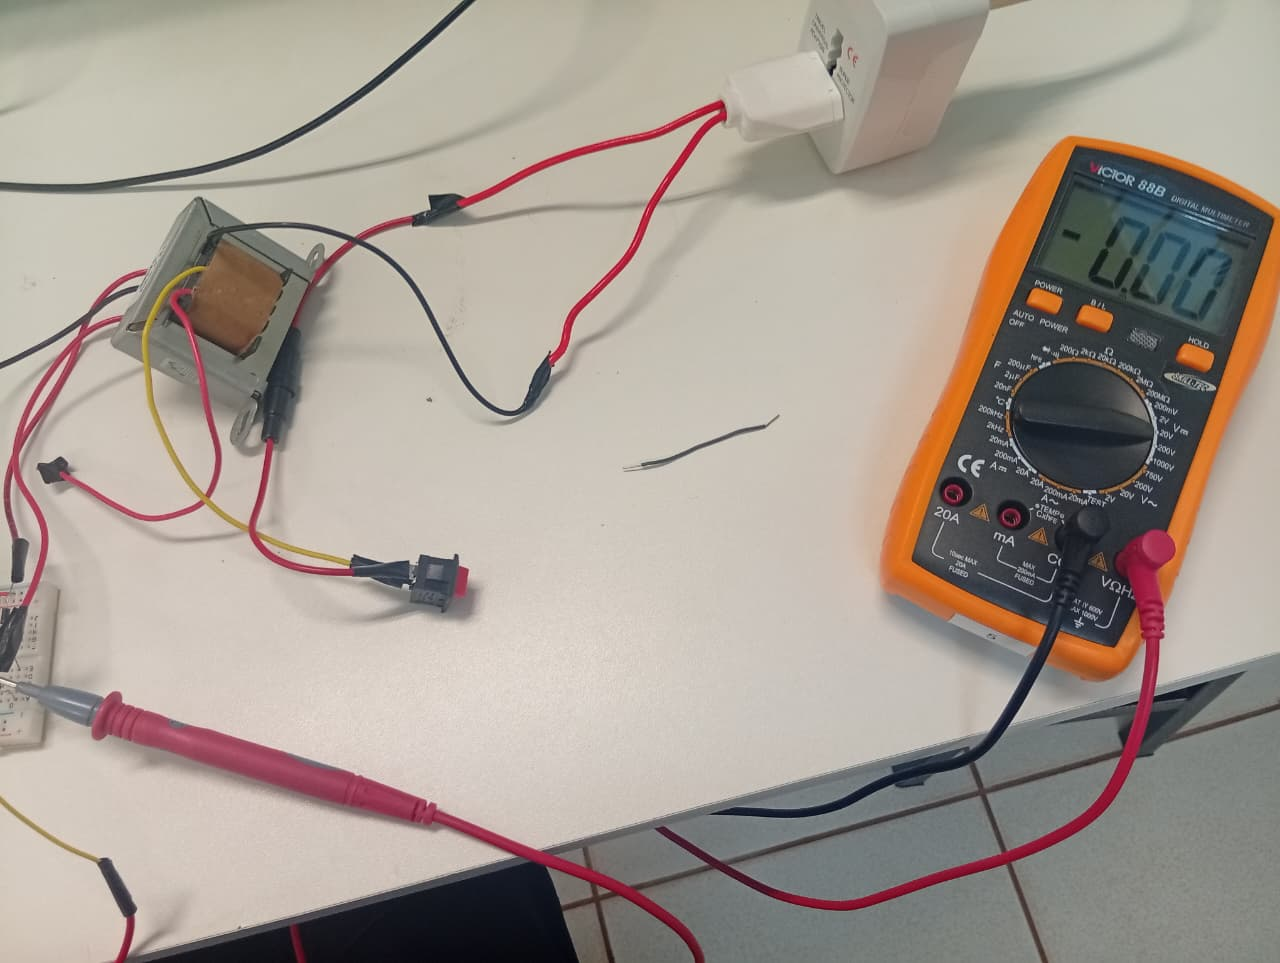
\includegraphics[width=\columnwidth,height=5.6cm,keepaspectratio]{Images/exp1_multimetro.jpeg}
\caption{Experimento 1 --- Multímetro Victor 88B com seletor na escala $20\,\text{V}$ DC, indicando $0{,}00\,\text{V}$. A função correta para o ensaio era V$\sim$ (procedimento incorreto).}
\label{fig:exp1-multi}
\end{figure}

\begin{figure}[H]
\centering
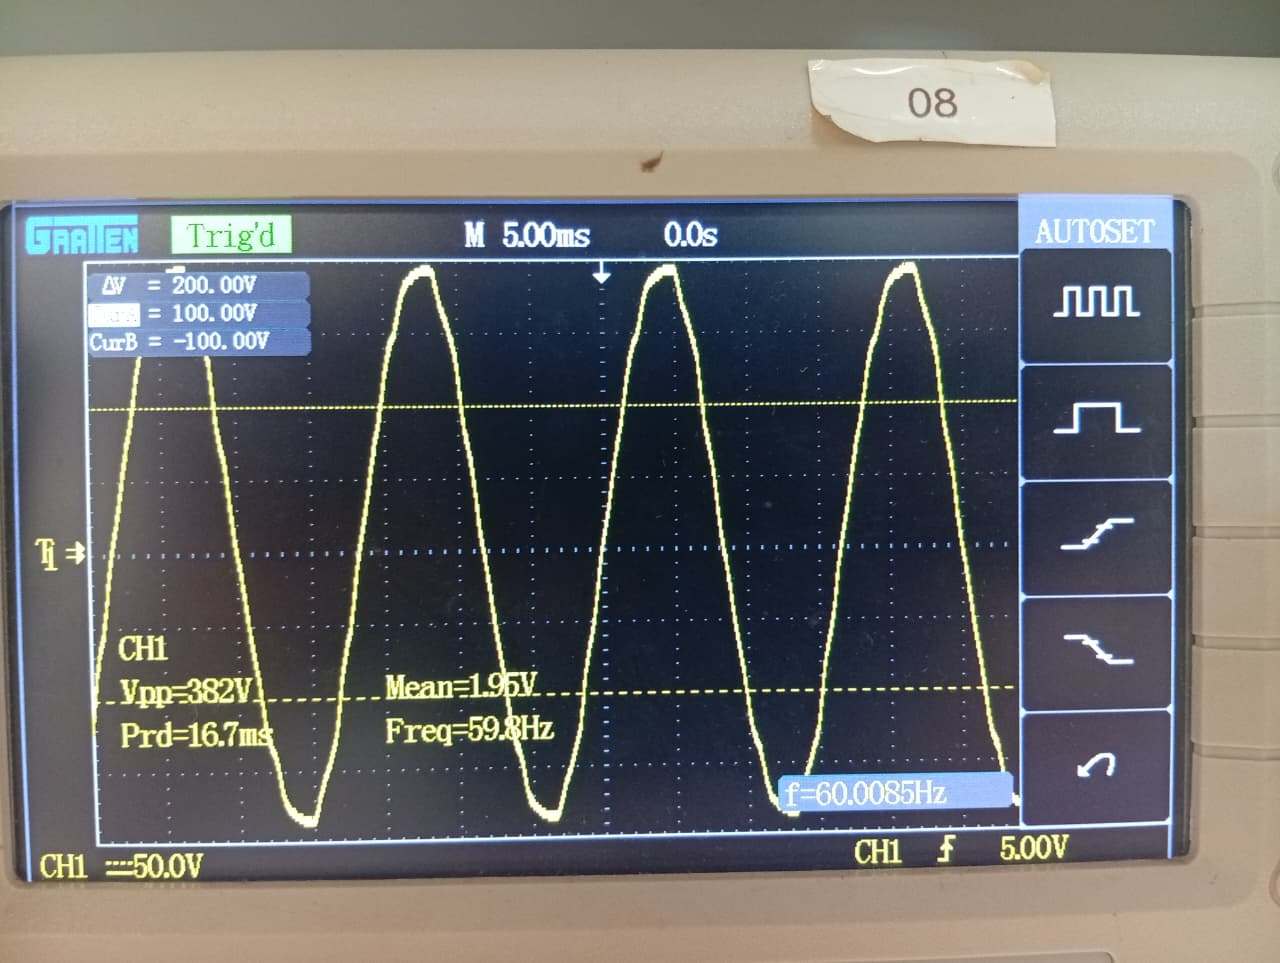
\includegraphics[width=\columnwidth,height=5.6cm,keepaspectratio]{Images/exp1_osciloscopio.jpeg}
\caption{Experimento 1 --- Secundário do transformador ($5{,}00\,\text{ms/div}$, $50{,}0\,\text{V/div}$ exibidos, acoplamento DC, canal em $10\times$ com ponta em $1\times$). Exibido: $V_{\text{pp}} = 382\,\text{V}$; real (fator $1/10$): $38{,}2\,\text{V}$. Contador: $60{,}01\,\text{Hz}$.}
\label{fig:exp1-osc}
\end{figure}

\textbf{Valor exibido e fator.} No osciloscópio (Figura~\ref{fig:exp1-osc}), em modo \textit{Trig'd}, acoplamento DC e \textit{trigger} em $5{,}00\,\text{V}$, o visor indica $V_{\text{pp}} = 382\,\text{V}$ em $50{,}0\,\text{V/div}$, $\text{Mean} = 1{,}95\,\text{V}$, $\text{Prd} = 16{,}7\,\text{ms}$ e $\text{Freq} = 59{,}8\,\text{Hz}$. O canal estava configurado em $10\times$ com a ponta em $1\times$; o valor exibido é, portanto, $10$ vezes o valor real (fator $1/10$). Essa atenuação é coerente com a leitura posterior de $19{,}1\,\text{V}$ de pico no Experimento~2A, obtida com fator $1\times$.

\textbf{Valor real.}
\begin{equation}
V_{\text{pp,real}} = \frac{382\,\text{V}}{10} = 38{,}2\,\text{V}, \qquad V_{p,\text{real}} = \frac{38{,}2\,\text{V}}{2} = 19{,}1\,\text{V}.
\end{equation}
Pela Eq.~\eqref{eq:vpico}, o valor eficaz em vazio é
\begin{equation}
V_{\text{RMS}} = \frac{19{,}1}{\sqrt{2}} \approx 13{,}5\,\text{V},
\end{equation}
valor obtido do osciloscópio, que supõe forma de onda senoidal. O $\text{Mean}$ exibido de $1{,}95\,\text{V}$ corresponde a $0{,}195\,\text{V}$ reais; a janela de $60\,\text{ms}$ (12 divisões de $5{,}00\,\text{ms}$) equivale a $3{,}6$ períodos, o que pode deixar a média da janela diferente de zero (hipótese, não verificada).

\textbf{Esperado e desvio.} Para $12\,\text{V}$ RMS nominais, $V_{\text{RMS}} = 13{,}5\,\text{V}$ representa $+12{,}5\%$. A especificação do trabalho refere-se à tensão nominal do transformador; o valor em vazio é maior que o nominal. Não foi verificado o valor sob carga. A frequência medida no osciloscópio ($59{,}8\,\text{Hz}$, desvio de $-0{,}33\%$ em relação a $60\,\text{Hz}$) tem resolução limitada pelo período exibido ($0{,}1\,\text{ms}$ em $16{,}7\,\text{ms}$); o contador indica $60{,}01\,\text{Hz}$ ($+0{,}01\%$). Observam-se cristas levemente achatadas na forma de onda; a causa não foi investigada.

\textbf{Multímetro.} Com o seletor em $20\,\text{V}$ DC (Figura~\ref{fig:exp1-multi}), o visor indicou $0{,}00\,\text{V}$. Esse valor decorre de falha de procedimento: a medição de tensão alternada exigia a função V$\sim$. A leitura não é resultado do ensaio, e nenhuma medição AC foi obtida com o multímetro.

\subsection{Experimento 2 --- Onda Pós-Diodos (Sem e Com Filtro Capacitivo)}

\textbf{Condição.} Na etapa A, o capacitor de $4700\,\mu\text{F}$ foi removido e um resistor de $1\,\text{k}\Omega$ foi conectado do nó pós-fusível ao GND. Na etapa B, o resistor foi retirado e o capacitor foi reinstalado. As Figuras~\ref{fig:exp2-sem-cap-proto} e~\ref{fig:exp2-sem-cap-osc} referem-se à etapa A, e as Figuras~\ref{fig:exp2-com-cap-proto} e~\ref{fig:exp2-com-cap-osc}, à etapa B.

\begin{figure}[H]
\centering
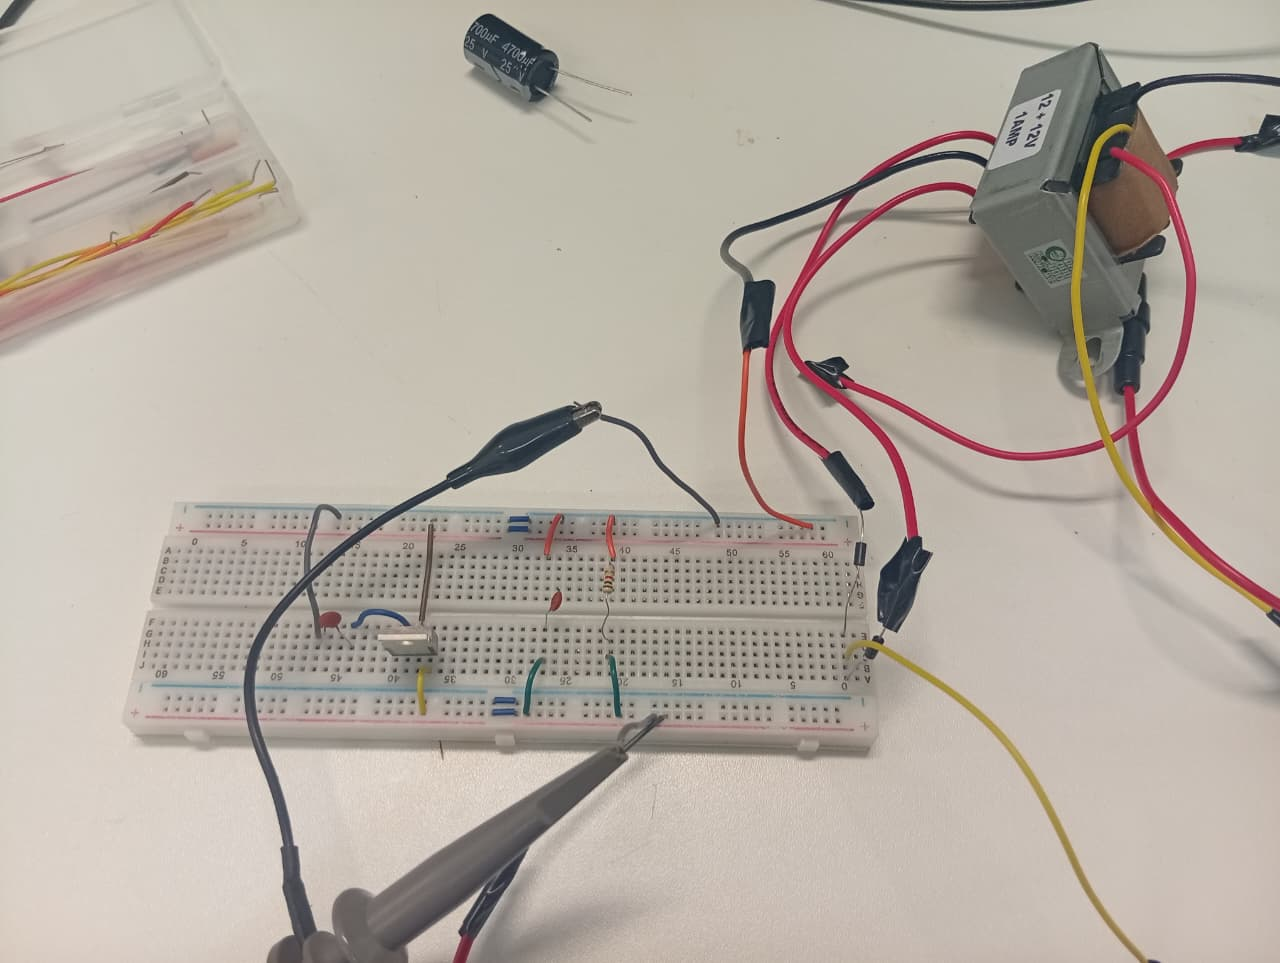
\includegraphics[width=\columnwidth,height=5.6cm,keepaspectratio]{Images/exp2_protoboard-osciloscopio_com-resistencia-1k-ohm.jpeg}
\caption{Experimento 2 (etapa A) --- Montagem sem o capacitor de $4700\,\mu\text{F}$ e com resistor de $1\,\text{k}\Omega$ até o GND.}
\label{fig:exp2-sem-cap-proto}
\end{figure}

\begin{figure}[H]
\centering
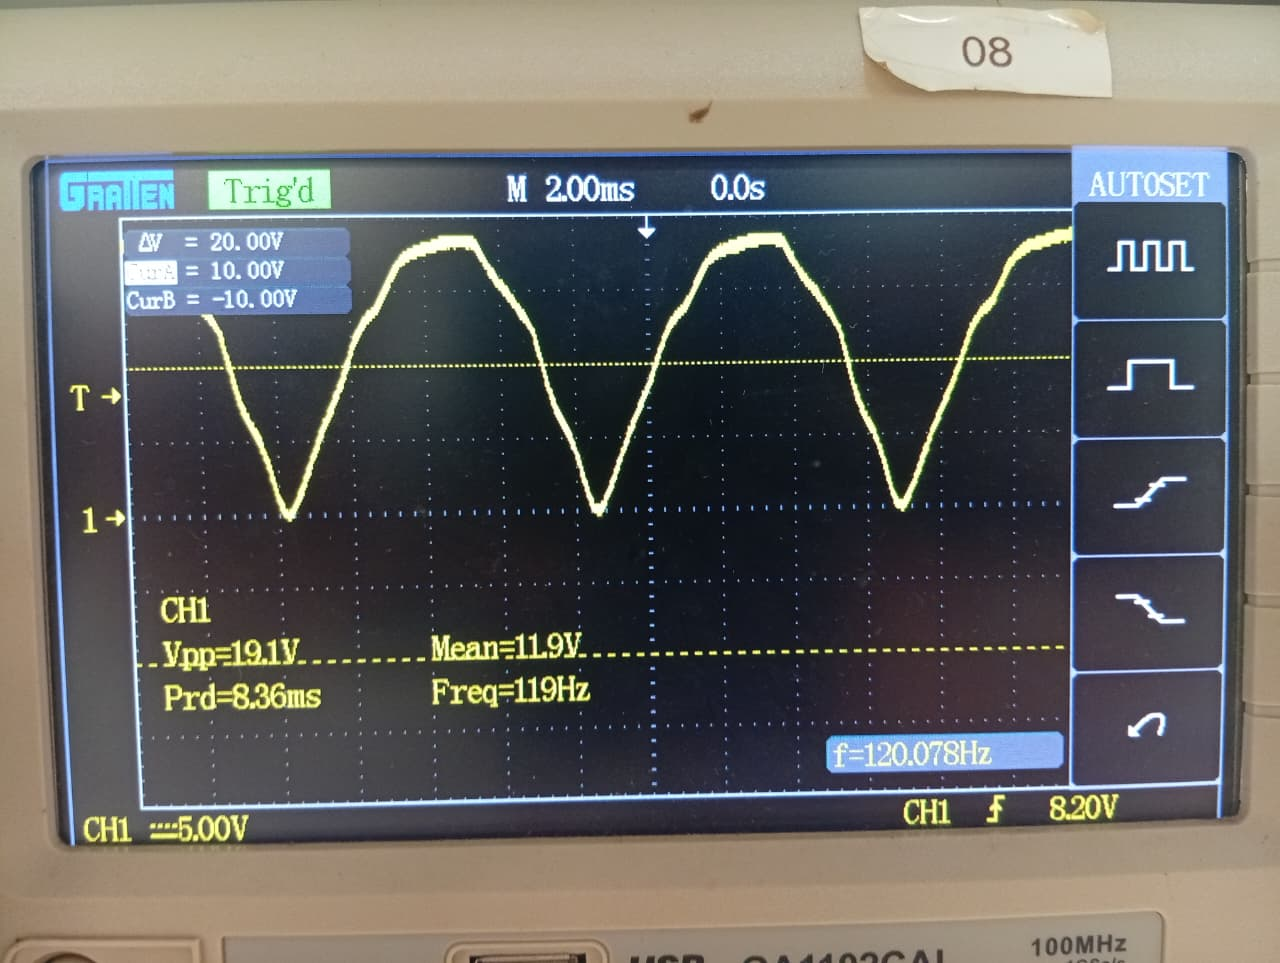
\includegraphics[width=\columnwidth,height=5.6cm,keepaspectratio]{Images/exp2_osciloscopio_com-resistencia-1k-ohm.jpeg}
\caption{Experimento 2 (etapa A) --- Onda retificada sem filtro, acoplamento DC, $5{,}00\,\text{V/div}$, $2{,}00\,\text{ms/div}$, fator $1\times$ (valor real igual ao exibido): $V_{\text{pp}} = 19{,}1\,\text{V}$, $\text{Mean} = 11{,}9\,\text{V}$; contador: $120{,}08\,\text{Hz}$.}
\label{fig:exp2-sem-cap-osc}
\end{figure}

\begin{figure}[H]
\centering
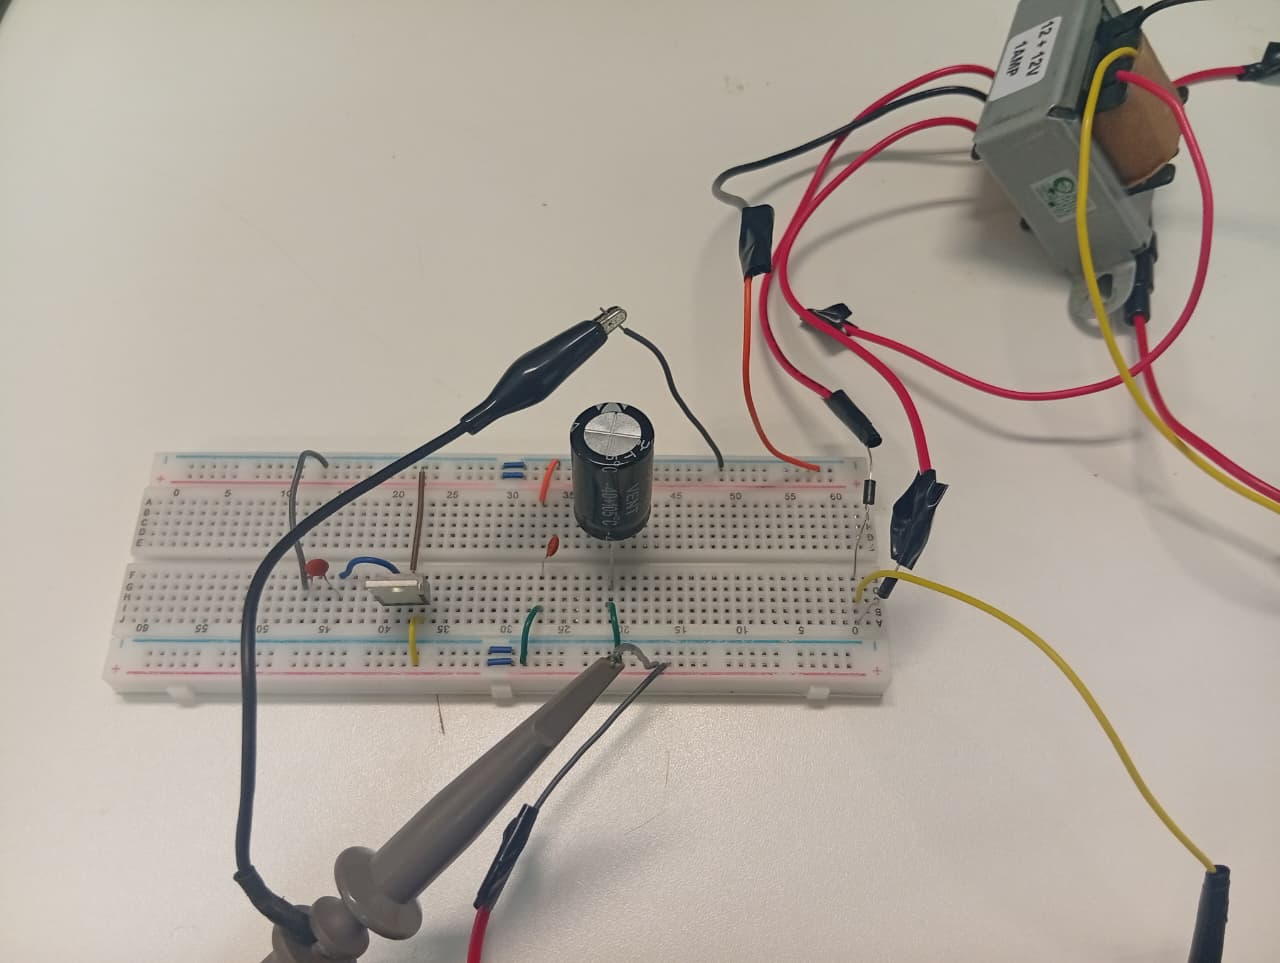
\includegraphics[width=\columnwidth,height=5.6cm,keepaspectratio]{Images/exp2_protoboard-osciloscopio_com-capacitor.jpeg}
\caption{Experimento 2 (etapa B) --- Montagem após a retirada do resistor de $1\,\text{k}\Omega$ e a reinserção do capacitor de $4700\,\mu\text{F}$.}
\label{fig:exp2-com-cap-proto}
\end{figure}

\begin{figure}[H]
\centering
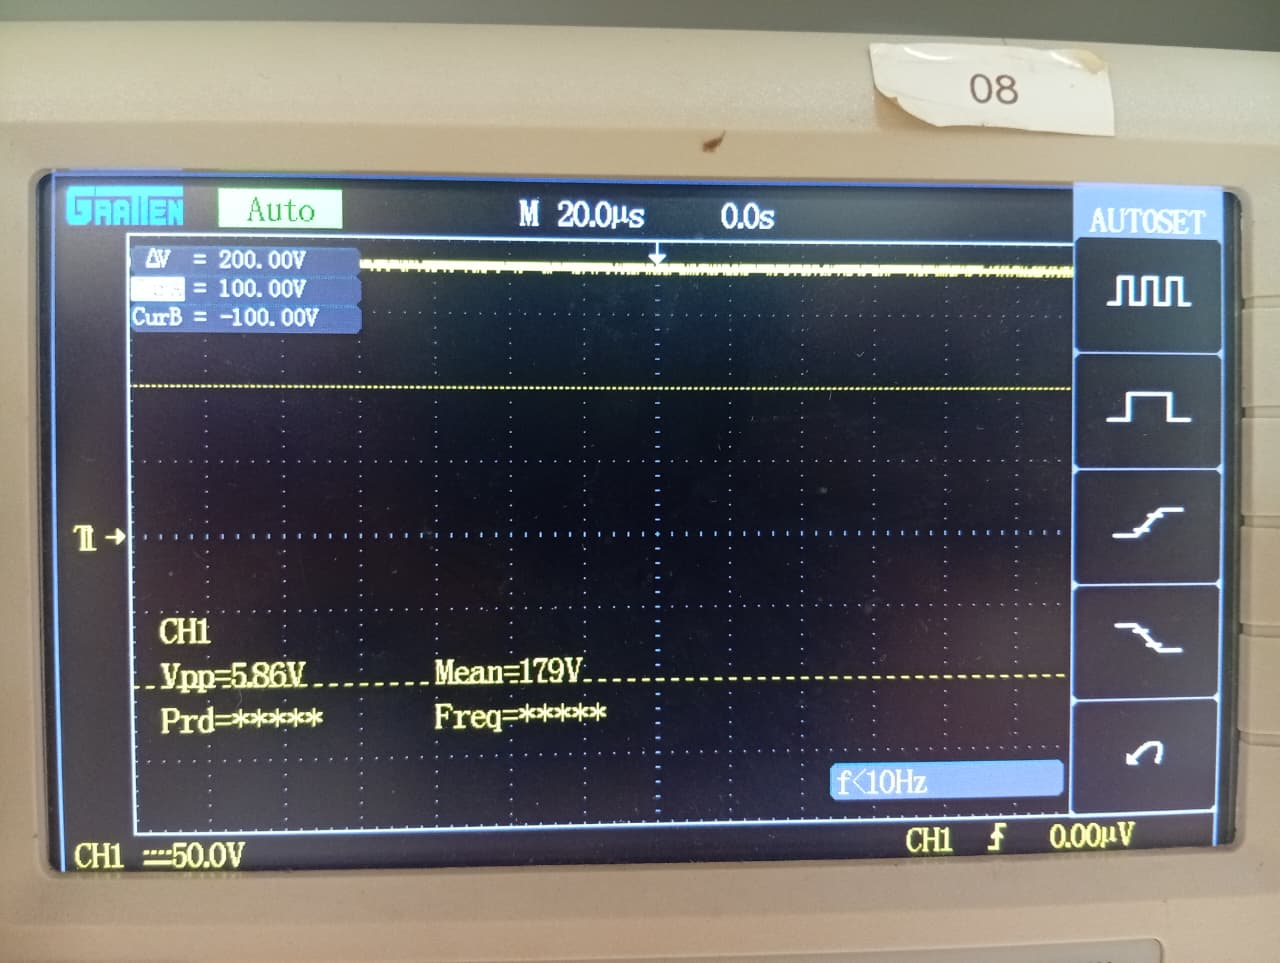
\includegraphics[width=\columnwidth,height=5.6cm,keepaspectratio]{Images/exp2_osciloscopio_com-capacitor.jpeg}
\caption{Experimento 2 (etapa B) --- Captura com filtro capacitivo, acoplamento DC, $50{,}0\,\text{V/div}$ exibidos, $20{,}0\,\mu\text{s/div}$, modo \textit{Auto}, canal em $10\times$ com ponta em $1\times$. Exibido: $\text{Mean} = 179\,\text{V}$; real (fator $1/10$): $\approx 17{,}9\,\text{V}$.}
\label{fig:exp2-com-cap-osc}
\end{figure}

\textbf{Etapa A --- valor exibido, fator e real.} Com $5{,}00\,\text{V/div}$, $2{,}00\,\text{ms/div}$, fator $1\times$ e \textit{trigger} em $8{,}20\,\text{V}$ (Figura~\ref{fig:exp2-sem-cap-osc}), observam-se semiciclos positivos sucessivos a partir da referência de $0\,\text{V}$, o que é compatível com a retificação de onda completa. Os valores exibidos, que coincidem com os reais, são $V_{\text{pp}} = 19{,}1\,\text{V}$, $\text{Mean} = 11{,}9\,\text{V}$, $\text{Prd} = 8{,}36\,\text{ms}$ e $\text{Freq} = 119\,\text{Hz}$; o contador indica $120{,}08\,\text{Hz}$. O período de $8{,}36\,\text{ms}$ difere em $+0{,}3\%$ dos $8{,}33\,\text{ms}$ esperados para $120\,\text{Hz}$.

\textbf{Esperado e desvio.} Com a Eq.~\eqref{eq:vdc_sem_filtro} aplicada a dois valores de pico:
\begin{equation}
V_{\text{DC}} = \frac{2 \times 19{,}1}{\pi} \approx 12{,}16\,\text{V} \quad (V_{p,\text{ret}} = 19{,}1\,\text{V}),
\end{equation}
com desvio $(11{,}9 - 12{,}16)/12{,}16 \approx -2{,}1\%$; e
\begin{equation}
V_{\text{DC}} = \frac{2 \times 18{,}4}{\pi} \approx 11{,}71\,\text{V} \quad (V_{p,\text{ret}} = 19{,}1 - 0{,}7 = 18{,}4\,\text{V}),
\end{equation}
com desvio $(11{,}9 - 11{,}71)/11{,}71 \approx +1{,}6\%$. A média medida concorda com os dois cálculos dentro de $\approx \pm 2\%$, compatível com a resolução de $5\,\text{V/div}$ e com a variação da rede. O desvio não é atribuído à condução dos diodos.

\textbf{Observações sobre os picos.} O pico pós-diodo ($19{,}1\,\text{V}$) é igual ao pico medido antes do diodo no Experimento~1 ($19{,}1\,\text{V}$), embora se espere um valor $\approx 0{,}7\,\text{V}$ menor, isto é, $18{,}4\,\text{V}$. Além disso, os $17{,}96\,\text{V}$ DC com capacitor (Experimento~3) ficam $\approx 1{,}1\,\text{V}$ abaixo de $19{,}1\,\text{V}$ e $\approx 0{,}44\,\text{V}$ abaixo de $18{,}4\,\text{V}$. Como hipótese, não verificada, essas diferenças podem decorrer de variação da rede entre as capturas e da resolução de leitura do osciloscópio; a causa não pôde ser determinada.

\textbf{Etapa B --- valor exibido, fator e real.} Com $50{,}0\,\text{V/div}$, $20{,}0\,\mu\text{s/div}$ e modo \textit{Auto} (Figura~\ref{fig:exp2-com-cap-osc}), o visor indica $\text{Mean} = 179\,\text{V}$ e $V_{\text{pp}} = 5{,}86\,\text{V}$; o contador indica $f < 10\,\text{Hz}$. Com a atenuação $10\times$ (canal em $10\times$ com ponta em $1\times$, fator $1/10$), o valor real é $\text{Mean} \approx 17{,}9\,\text{V}$, diferença de $-0{,}06\,\text{V}$ ($-0{,}3\%$) em relação aos $17{,}96\,\text{V}$ medidos no multímetro no Experimento~3. O valor de $V_{\text{pp}}$ exibido ($5{,}86\,\text{V}$, ou $0{,}586\,\text{V}$ com o fator $1/10$) não é utilizado como resultado, e sua origem não foi determinada.

A janela temporal corresponde a $20\,\mu\text{s/div} \times 12\ \text{divisões visíveis} = 240\,\mu\text{s}$, cerca de $2{,}9\%$ do período de $8{,}33\,\text{ms}$. Essa base de tempo não permite observar o \textit{ripple} nem medir período ou frequência. O resultado válido desta etapa é o nível DC de $\approx 17{,}9\,\text{V}$, confirmado pelo multímetro.

\subsection{Experimento 3 --- Filtro e \textit{Ripple} antes do LM7812 (Pino 1)}

\textbf{Condição.} Mediram-se a tensão DC e a ondulação no pino~1 do LM7812. As Figuras~\ref{fig:exp3-proto} e~\ref{fig:exp3-multi} referem-se à leitura DC, e as Figuras~\ref{fig:exp3-sem-led-osc} e~\ref{fig:exp3-com-led-osc} mostram o \textit{ripple} em acoplamento AC ($2{,}00\,\text{mV/div}$, $5{,}00\,\text{ms/div}$, limite de banda B e filtro F ativos) sem carga na saída e com LED + $1\,\text{k}\Omega$.

\begin{figure}[H]
\centering
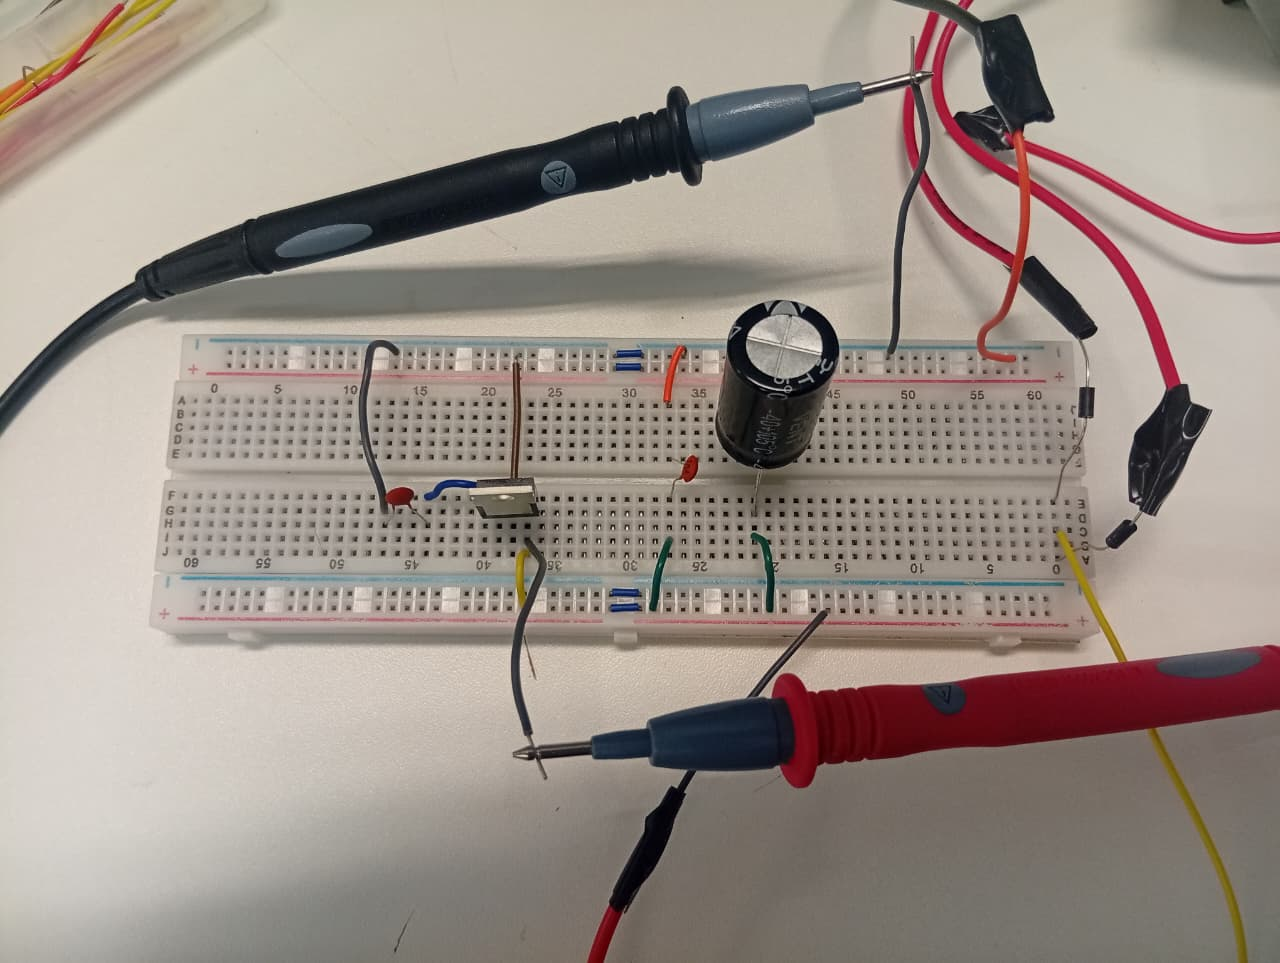
\includegraphics[width=\columnwidth,height=5.6cm,keepaspectratio]{Images/exp3_protoboard-multimetro.jpeg}
\caption{Experimento 3 --- Montagem para medição no pino~1 do LM7812.}
\label{fig:exp3-proto}
\end{figure}

\begin{figure}[H]
\centering
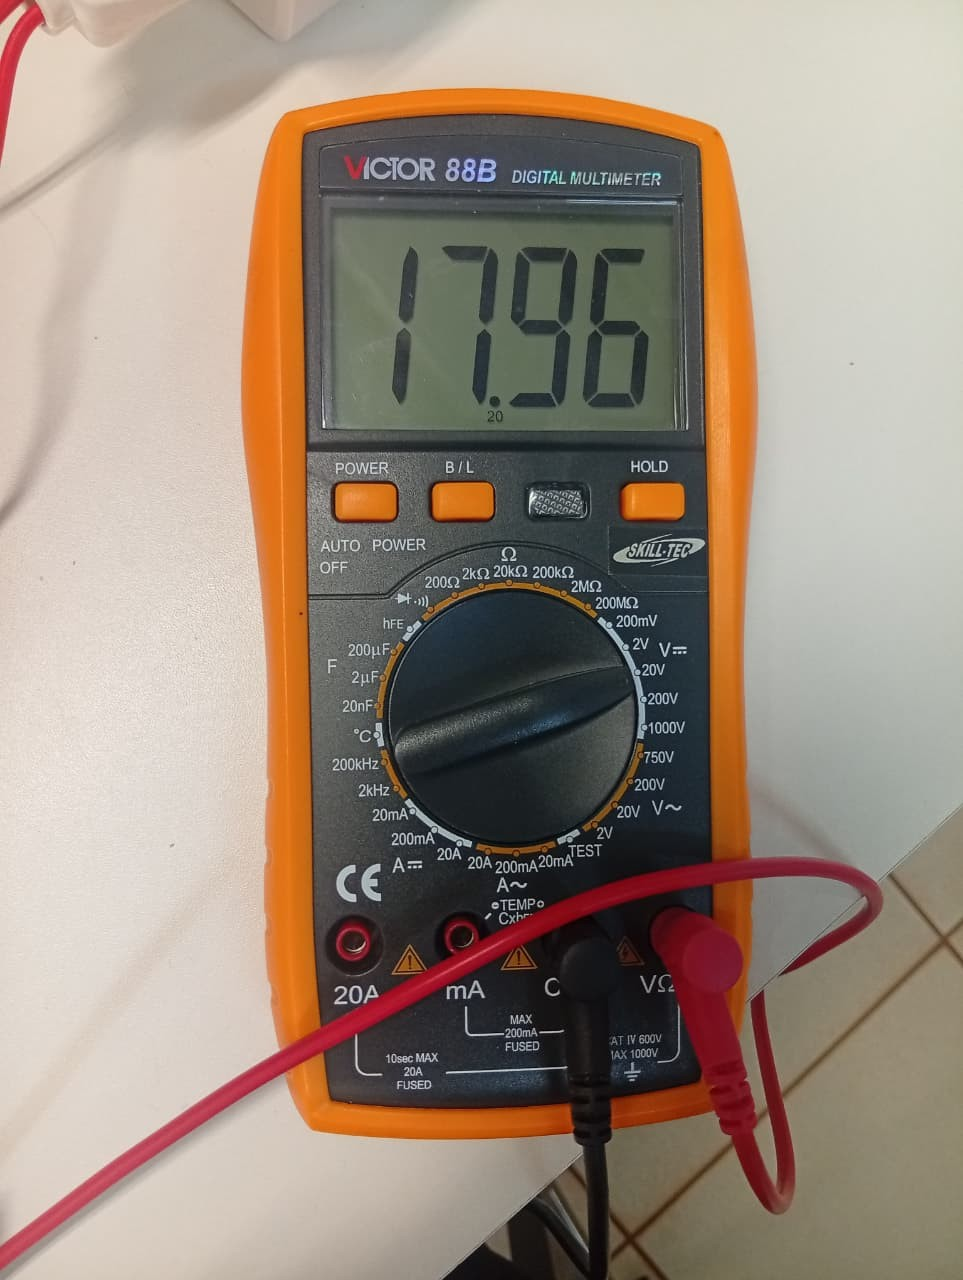
\includegraphics[width=\columnwidth,height=5.6cm,keepaspectratio]{Images/exp3_multimetro.jpeg}
\caption{Experimento 3 --- Multímetro Victor 88B na escala $20\,\text{V}$ DC indicando $17{,}96\,\text{V}$ no pino~1 do LM7812.}
\label{fig:exp3-multi}
\end{figure}

%% Foto de montagem repetida (uma foto de montagem por experimento e mantida na Figura anterior).
%\begin{figure}[H]
%\centering
%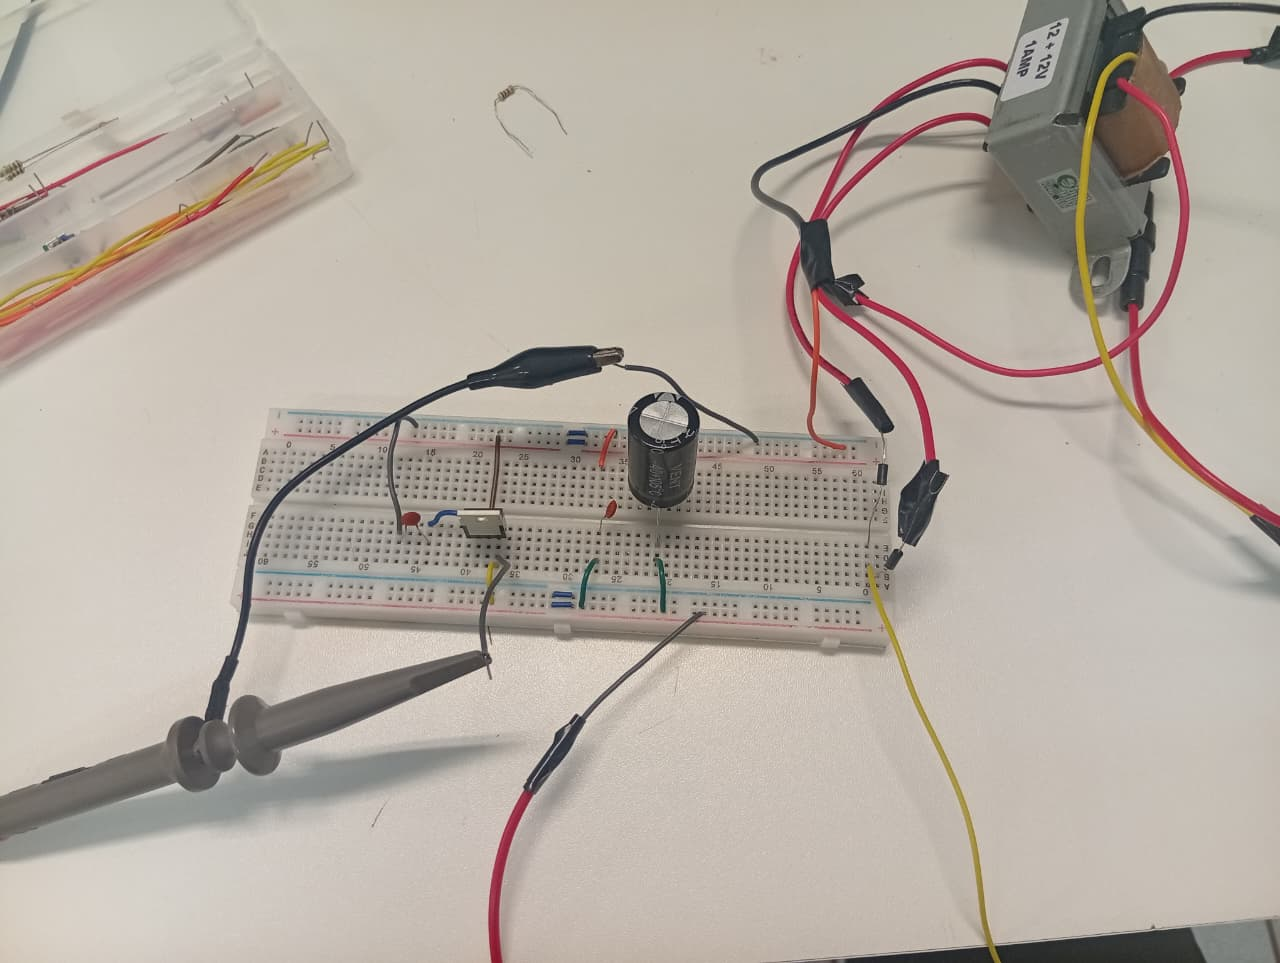
\includegraphics[width=\columnwidth,height=5.6cm,keepaspectratio]{Images/exp3_protoboard-osciloscopio_sem-led-resistencia-1k-ohm.jpeg}
%\caption{Experimento 3 (etapa B) --- Medição no pino~1 do LM7812 sem carga externa na saída de $12\,\text{V}$.}
%\label{fig:exp3-sem-led-proto}
%\end{figure}

\begin{figure}[H]
\centering
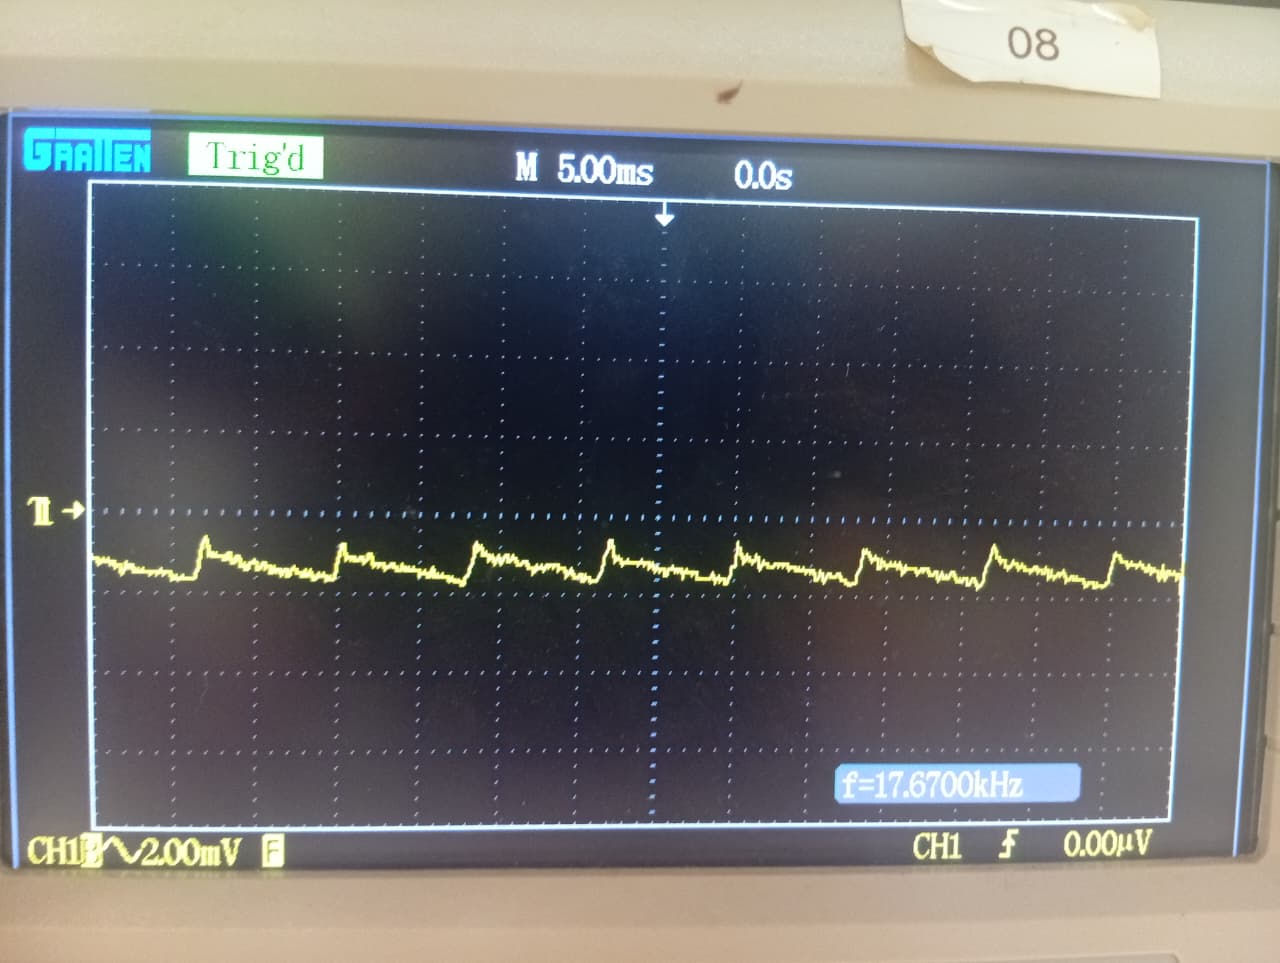
\includegraphics[width=\columnwidth,height=5.6cm,keepaspectratio]{Images/exp3_osciloscopio_sem-led-resistencia-1k-ohm.jpeg}
\caption{Experimento 3 --- Pino~1 sem carga na saída, acoplamento AC, $2{,}00\,\text{mV/div}$ exibidos, $5{,}00\,\text{ms/div}$, B e F ativos, fator da ponta não registrado: dente de serra de $\approx 0{,}6$ a $0{,}7\,\text{div}$, ou $\approx 1{,}2$ a $1{,}4\,\text{mV}_{\text{pp}}$ exibidos.}
\label{fig:exp3-sem-led-osc}
\end{figure}

%% Foto de montagem repetida.
%\begin{figure}[H]
%\centering
%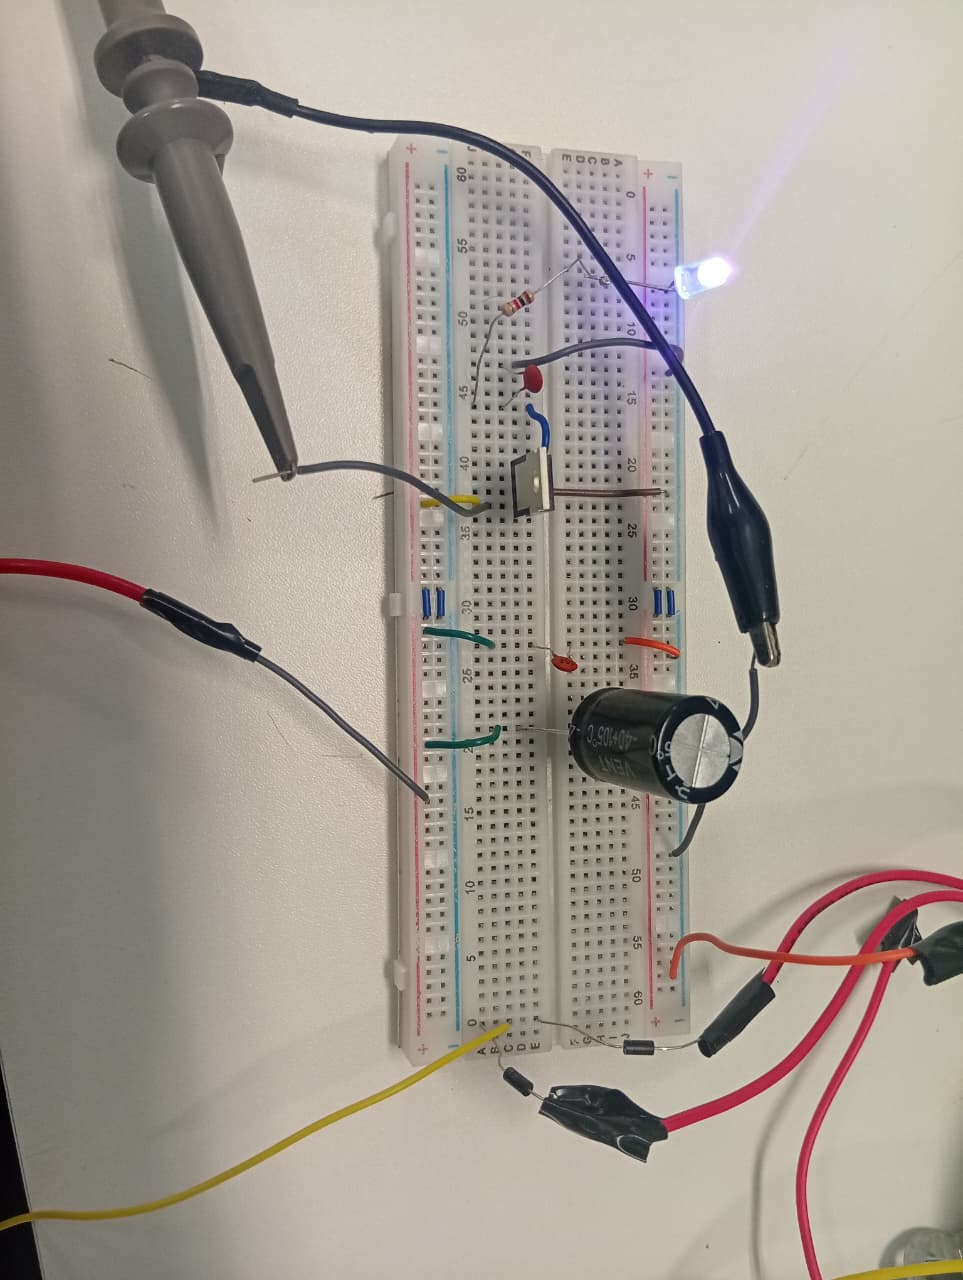
\includegraphics[width=\columnwidth,height=5.6cm,keepaspectratio]{Images/exp3_protoboard-osciloscopio_com-led-resistencia-1k-ohm.jpeg}
%\caption{Experimento 3 (etapa C) --- Medição no pino~1 do LM7812 com LED e resistor de $1\,\text{k}\Omega$ conectados na saída.}
%\label{fig:exp3-com-led-proto}
%\end{figure}

\begin{figure}[H]
\centering
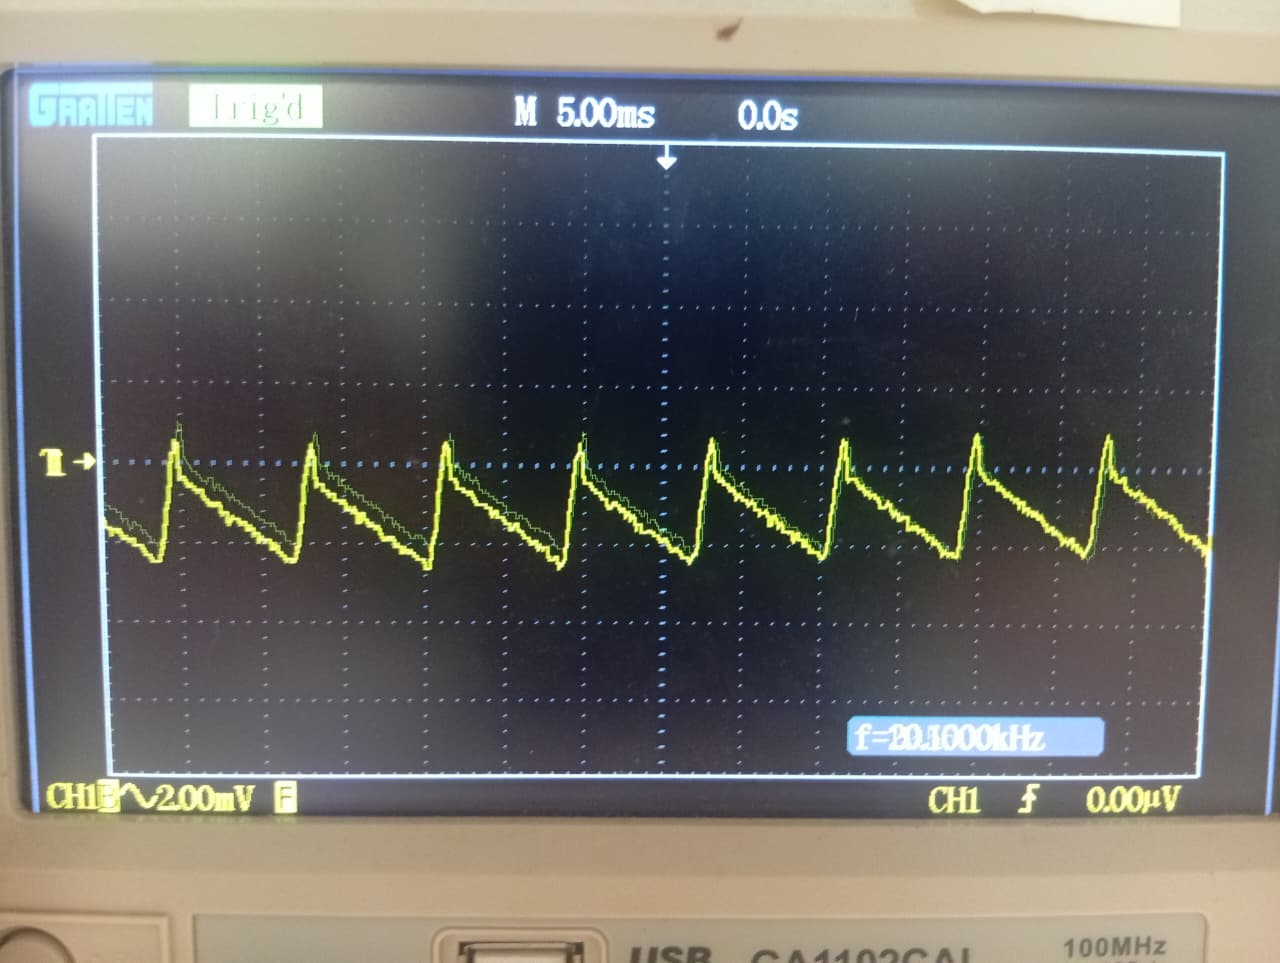
\includegraphics[width=\columnwidth,height=5.6cm,keepaspectratio]{Images/exp3_osciloscopio_com-led-resistencia-1k-ohm.jpeg}
\caption{Experimento 3 --- Pino~1 com LED + $1\,\text{k}\Omega$ na saída, acoplamento AC, $2{,}00\,\text{mV/div}$ exibidos, $5{,}00\,\text{ms/div}$, B e F ativos, fator da ponta não registrado: dente de serra de $\approx 1{,}4$ a $1{,}5\,\text{div}$, ou $\approx 2{,}8$ a $3{,}0\,\text{mV}_{\text{pp}}$ exibidos.}
\label{fig:exp3-com-led-osc}
\end{figure}

\textbf{Validado --- nível DC.} O multímetro (Figura~\ref{fig:exp3-multi}) indicou $17{,}96\,\text{V}$ DC, cerca de $6\,\text{V}$ acima da saída de $12\,\text{V}$ e cerca de $4\,\text{V}$ acima do mínimo de entrada de $14\,\text{V}$ ($12\,\text{V}$ + \textit{dropout} de $\approx 2\,\text{V}$, \textit{datasheet}~\cite{ds_lm7812}). O valor concorda com os $\approx 17{,}9\,\text{V}$ do Experimento~2B.

\textbf{Validado --- forma e crescimento relativo.} Nas Figuras~\ref{fig:exp3-sem-led-osc} e~\ref{fig:exp3-com-led-osc} observa-se forma de dente de serra, com subida rápida e descida gradual, e espaçamento de $\approx 1{,}67\,\text{div} \times 5{,}00\,\text{ms/div} = 8{,}33\,\text{ms}$ entre dentes, compatível com $120\,\text{Hz}$ (cerca de sete a oito dentes na janela de $60\,\text{ms}$). Os valores do contador ($17{,}67\,\text{kHz}$ e $20{,}10\,\text{kHz}$) são artefatos do nível de \textit{trigger} em $0{,}00\,\mu\text{V}$ e não representam a frequência do \textit{ripple}.

Pela Eq.~\eqref{eq:ripple}, com corrente quiescente de $\approx 5\,\text{mA}$ sem carga externa e $\approx 14\,\text{mA}$ com o LED, a razão de correntes é $14/5 = 2{,}8$. A razão das amplitudes lidas é $3{,}0/1{,}3 \approx 2{,}3$. O crescimento relativo com a carga é, portanto, coerente com o previsto. A corrente adicional do LED, $I_L \approx (11{,}95 - 3{,}0)/1000 \approx 9\,\text{mA}$, supõe $V_F \approx 3{,}0\,\text{V}$ (hipótese, não verificada; a tensão sobre o LED não foi medida).

\textbf{Não validado --- amplitude absoluta.} A Eq.~\eqref{eq:ripple} prevê
\begin{equation}
\Delta V_r \approx \frac{5\,\text{mA}}{120 \cdot 4700\,\mu\text{F}} \approx 8{,}9\,\text{mV}_{\text{pp}}
\end{equation}
sem carga externa e
\begin{equation}
\Delta V_r \approx \frac{14\,\text{mA}}{120 \cdot 4700\,\mu\text{F}} \approx 24{,}8\,\text{mV}_{\text{pp}}
\end{equation}
com o LED, contra $\approx 1{,}3$ e $\approx 3{,}0\,\text{mV}_{\text{pp}}$ lidos, isto é, valores lidos $\approx 7$ a $8$ vezes menores ($8{,}9/1{,}3 \approx 6{,}8$ e $24{,}8/3{,}0 \approx 8{,}3$), com desvios de $-85\%$ e $-88\%$. As causas possíveis, todas não verificadas, são: fator da ponta não registrado, filtro F, limite de banda B e valor de corrente quiescente de \textit{datasheet} diferente do real. A comparação quantitativa é inconclusiva, e a amplitude absoluta do \textit{ripple} não é considerada resultado validado.

\subsection{Experimento 4 --- Saída Regulada de $12\,\text{V}$ (Pino 3)}

\textbf{Condição.} Com o LED + $1\,\text{k}\Omega$ conectado na saída, mediram-se a tensão DC e o sinal residual no pino~3 (Figuras~\ref{fig:exp4-proto-multi} a~\ref{fig:exp4-osc}).

\begin{figure}[H]
\centering
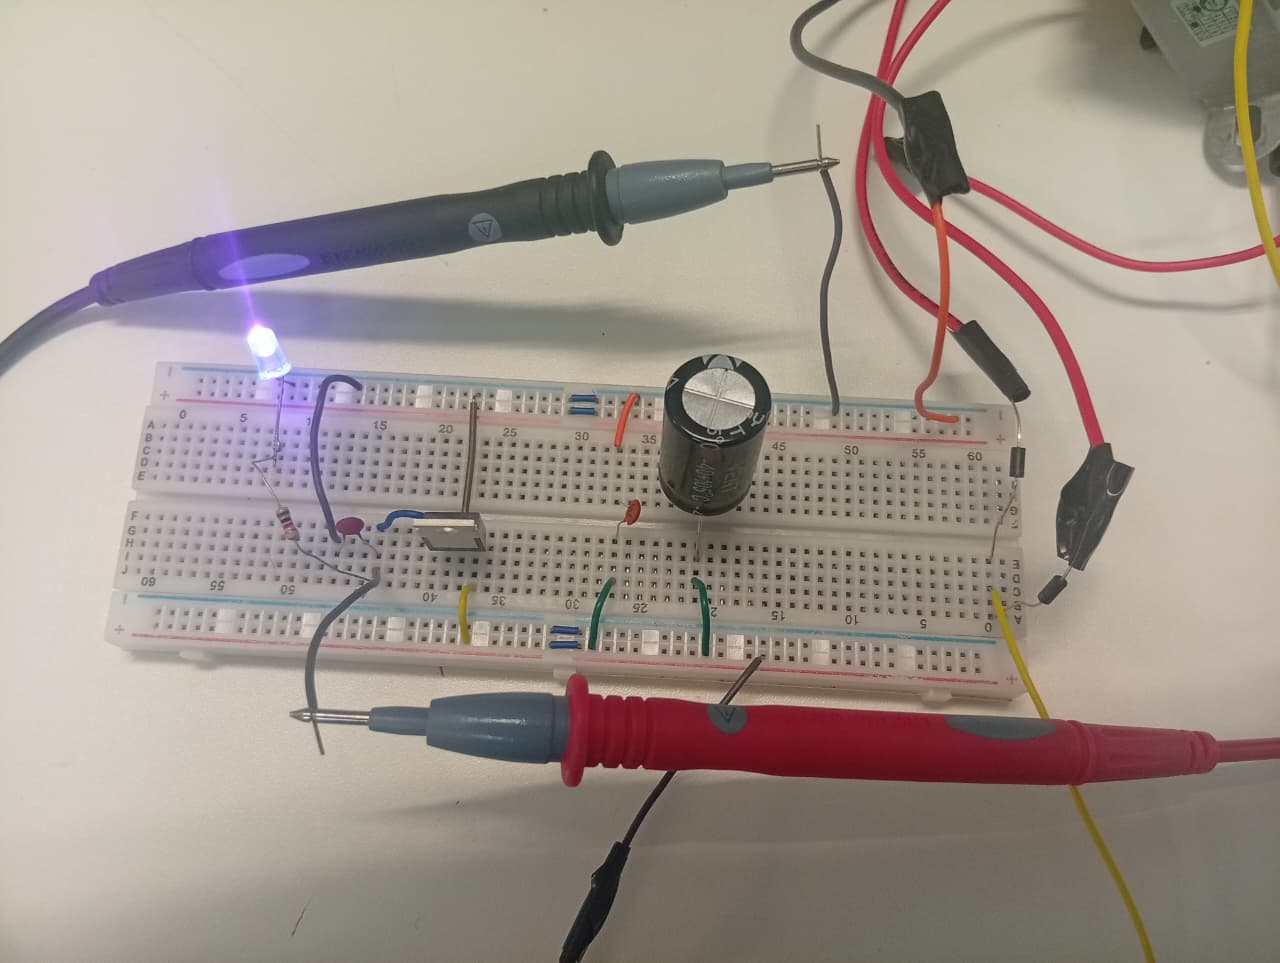
\includegraphics[width=\columnwidth,height=5.6cm,keepaspectratio]{Images/exp4_protoboard-multimetro.jpeg}
\caption{Experimento 4 --- Montagem com a medição no pino~3 do LM7812, com LED e resistor de $1\,\text{k}\Omega$ conectados.}
\label{fig:exp4-proto-multi}
\end{figure}

\begin{figure}[H]
\centering
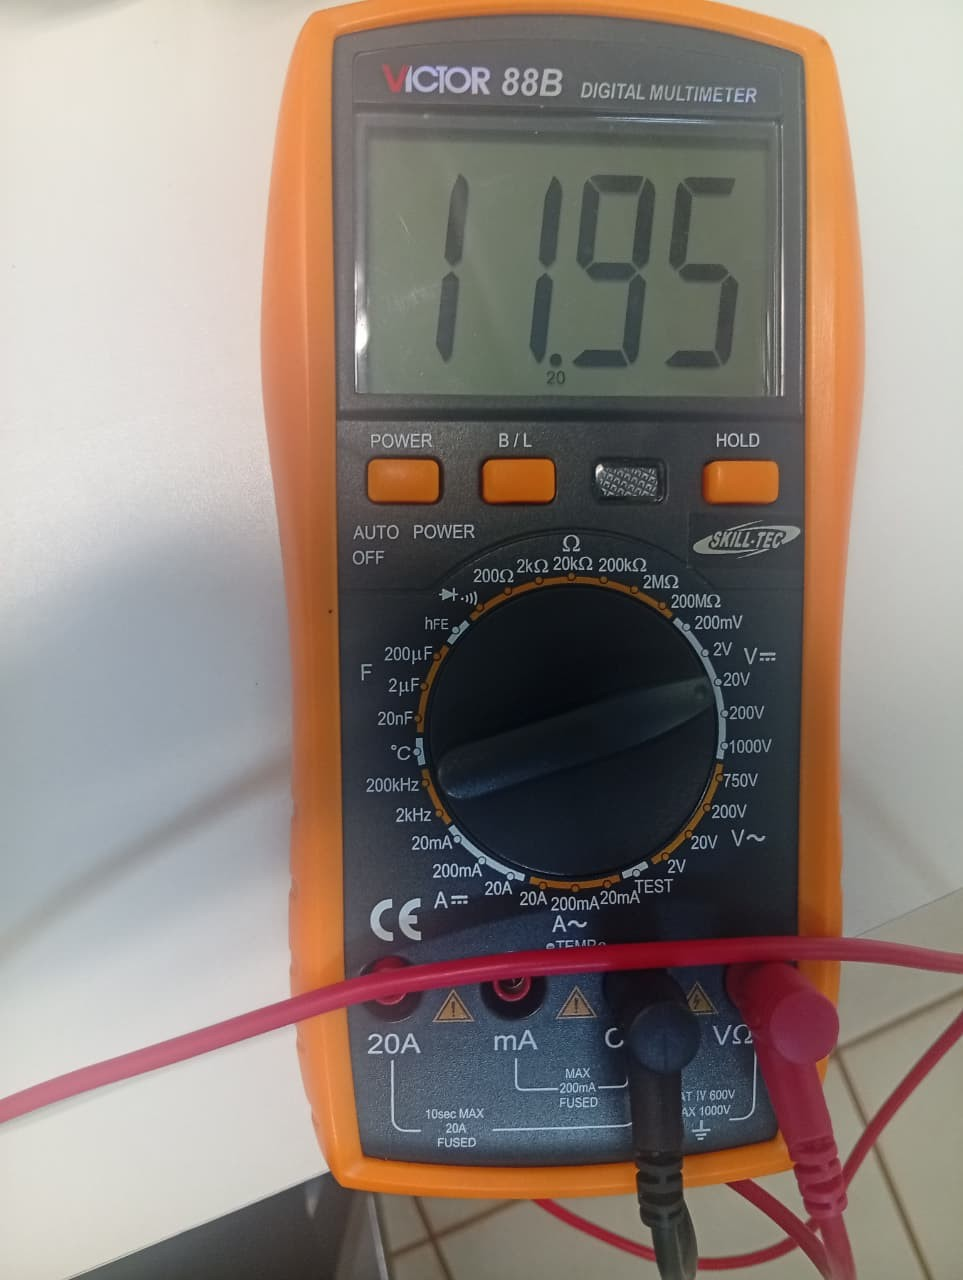
\includegraphics[width=\columnwidth,height=5.6cm,keepaspectratio]{Images/exp4_multimetro.jpeg}
\caption{Experimento 4 --- Multímetro Victor 88B na escala $20\,\text{V}$ DC indicando $11{,}95\,\text{V}$ na saída regulada.}
\label{fig:exp4-multi}
\end{figure}

%% Foto de montagem repetida.
%\begin{figure}[H]
%\centering
%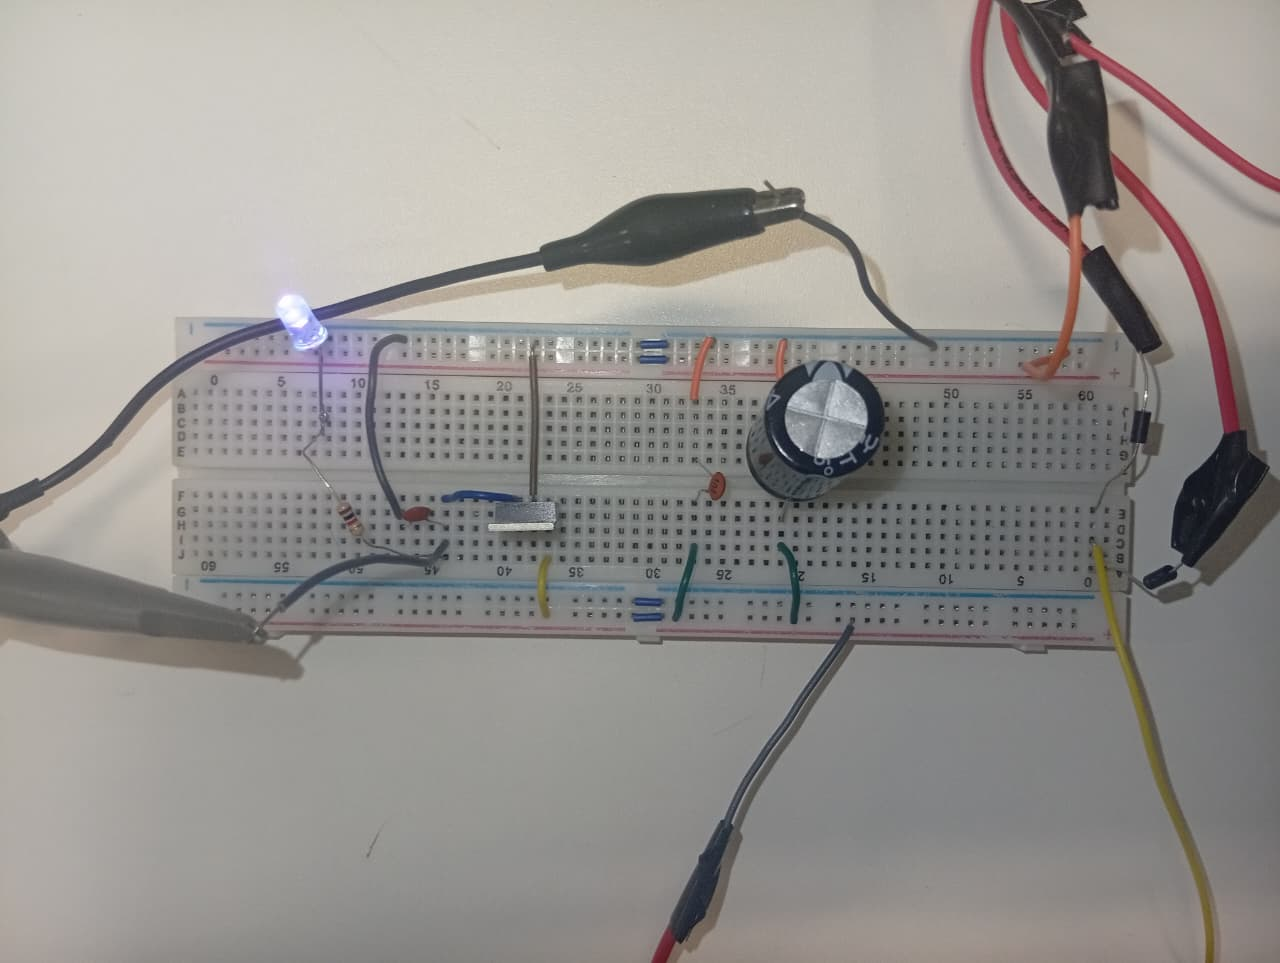
\includegraphics[width=\columnwidth,height=5.6cm,keepaspectratio]{Images/exp4_protoboard-osciloscopio.jpeg}
%\caption{Experimento 4 (etapa B) --- Ponta de prova do osciloscópio no pino~3 do LM7812 com carga ligada.}
%\label{fig:exp4-proto-osc}
%\end{figure}

\begin{figure}[H]
\centering
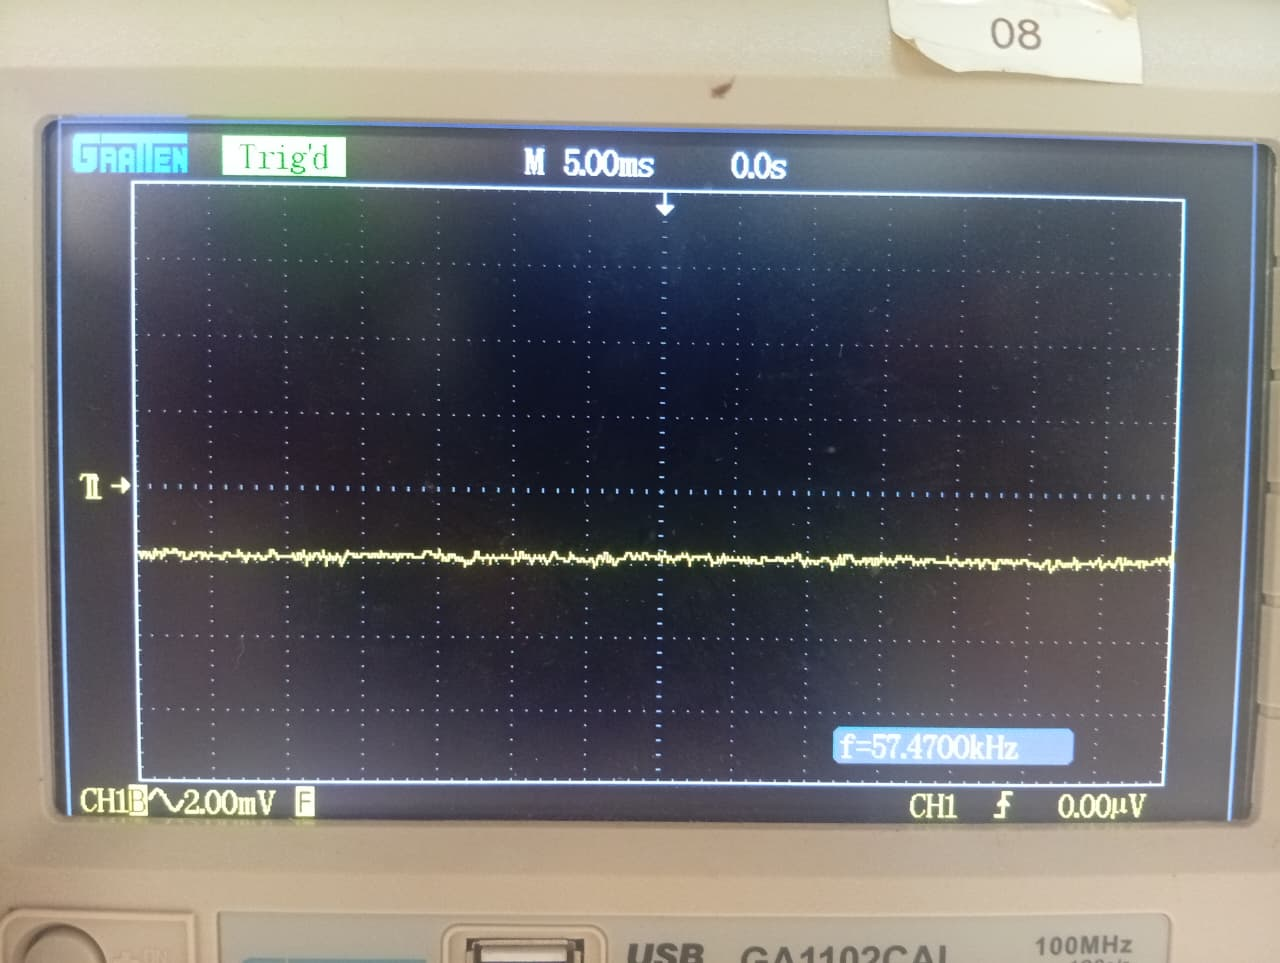
\includegraphics[width=\columnwidth,height=5.6cm,keepaspectratio]{Images/exp4_osciloscopio.jpeg}
\caption{Experimento 4 --- Saída de $12\,\text{V}$ com carga, acoplamento AC, $2{,}00\,\text{mV/div}$ exibidos, $5{,}00\,\text{ms/div}$, B e F ativos, fator da ponta não registrado: traço plano com piso de ruído $\lesssim 0{,}6\,\text{mV}_{\text{pp}}$ exibidos.}
\label{fig:exp4-osc}
\end{figure}

\textbf{Tensão.} O multímetro (Figura~\ref{fig:exp4-multi}) indicou $11{,}95\,\text{V}$ DC. Em relação a $12{,}00\,\text{V}$, o desvio é $(11{,}95 - 12{,}00)/12{,}00 \approx -0{,}42\%$, dentro da faixa de $\pm 4\%$ ($11{,}5\,\text{V}$ a $12{,}5\,\text{V}$, conforme \href{https://www.ti.com/lit/ds/symlink/lm340.pdf}{Datasheet do LM7812}) adotada como critério.

\textbf{\textit{Ripple}.} No osciloscópio (Figura~\ref{fig:exp4-osc}), com a mesma escala vertical, o mesmo acoplamento e a mesma base de tempo do Experimento~3, o traço permanece plano, sem o dente de serra de $120\,\text{Hz}$ do pino~1, com piso de ruído $\lesssim 0{,}6\,\text{mV}_{\text{pp}}$ exibidos. O valor de $57{,}47\,\text{kHz}$ do contador é artefato do \textit{trigger} e não representa sinal na saída. Esse piso é o limite de leitura, e não o valor do \textit{ripple} de saída.

Tomando os valores exibidos nas mesmas configurações, a relação entre a entrada ($\approx 3{,}0\,\text{mV}_{\text{pp}}$) e a saída ($\lesssim 0{,}6\,\text{mV}_{\text{pp}}$) corresponde a uma redução de $\approx 14$ a $16\,\text{dB}$ ($20\log(3{,}0/0{,}6) \approx 14\,\text{dB}$ e $20\log(3{,}0/0{,}5) \approx 15{,}6\,\text{dB}$). Esse valor é apenas um limite inferior, pois o piso de ruído limita a leitura e a configuração da ponta não foi validada. A rejeição de ondulação de $55$ a $70\,\text{dB}$ é valor de \href{https://www.ti.com/lit/ds/symlink/lm340.pdf}{Datasheet do LM7812} e não foi medida neste trabalho.

Os capacitores de $100\,\text{nF}$ não são responsáveis pela rejeição em $120\,\text{Hz}$: nessa frequência, sua reatância é $X_C = 1/(2\pi \cdot 120 \cdot 100\,\text{nF}) \approx 13\,\text{k}\Omega$. Eles servem à estabilidade do regulador e à atenuação de ruído de alta frequência.

\subsection{Experimento 5 --- Teste de Regulação de Carga}

\textbf{Condição.} O multímetro em $20\,\text{V}$ DC foi conectado entre o pino~3 e o GND sem carga (Figuras~\ref{fig:exp5-sem-led-proto} e~\ref{fig:exp5-sem-led-multi}) e com LED + $1\,\text{k}\Omega$ (Figura~\ref{fig:exp5-com-led-multi}).

\begin{figure}[H]
\centering
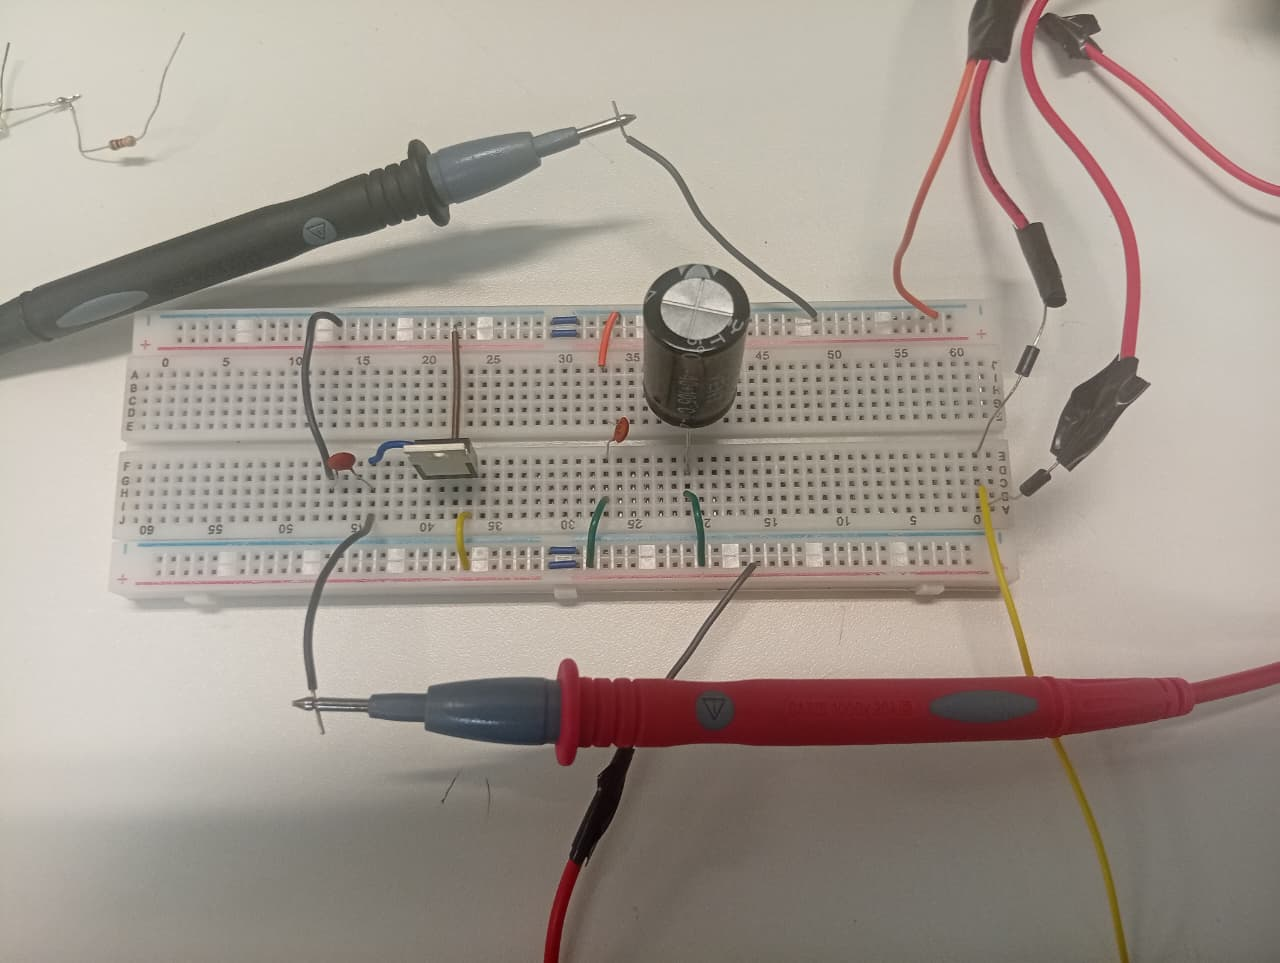
\includegraphics[width=\columnwidth,height=5.6cm,keepaspectratio]{Images/exp5_protoboard-multimetro_sem-led.jpeg}
\caption{Experimento 5 --- Montagem com o multímetro no pino~3, sem carga na saída (LED desconectado).}
\label{fig:exp5-sem-led-proto}
\end{figure}

\begin{figure}[H]
\centering
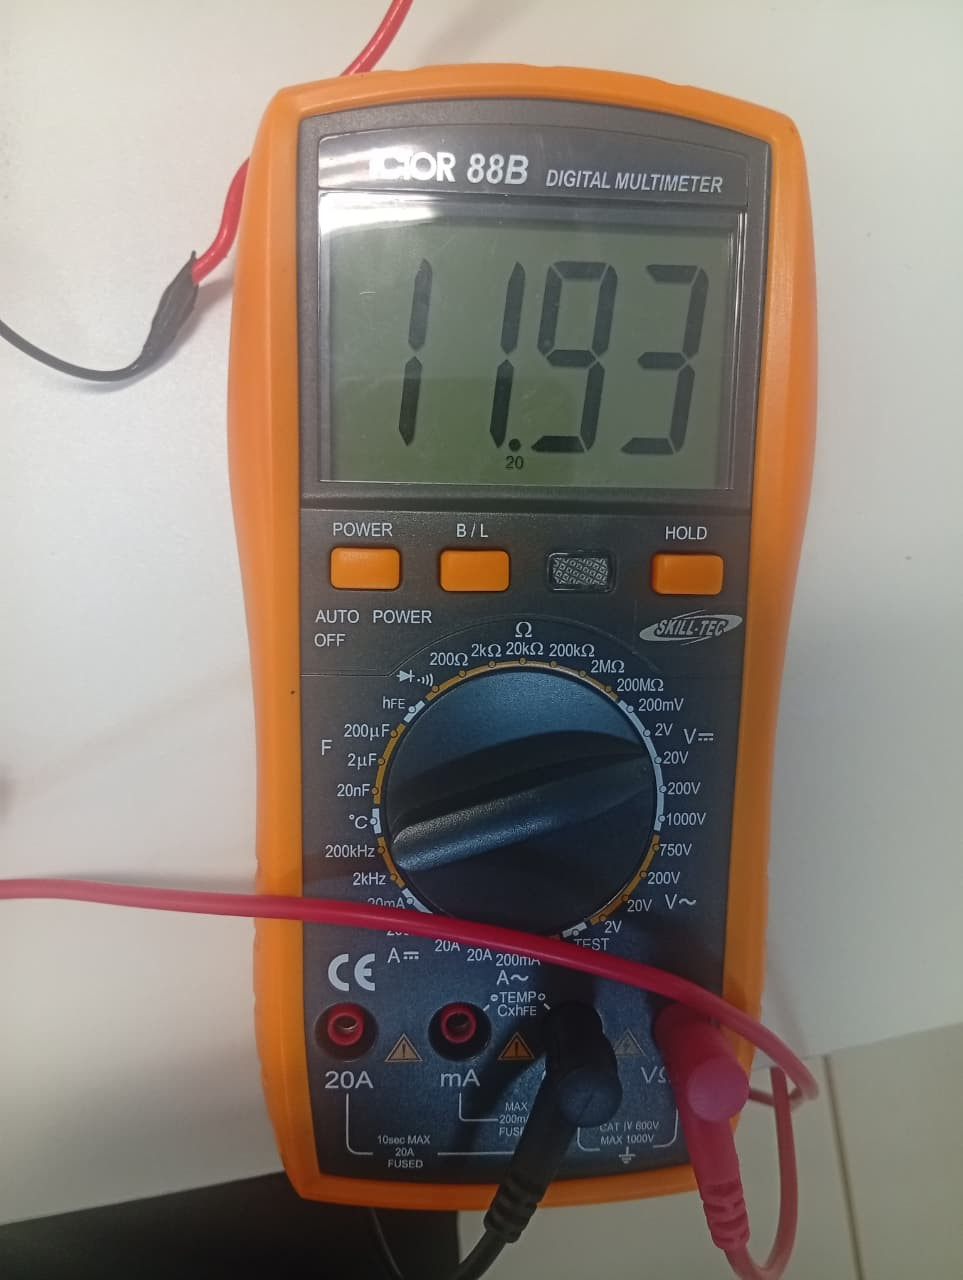
\includegraphics[width=\columnwidth,height=5.6cm,keepaspectratio]{Images/exp5_multimetro_sem-led.jpeg}
\caption{Experimento 5 --- Multímetro Victor 88B na escala $20\,\text{V}$ DC indicando $11{,}93\,\text{V}$ sem carga.}
\label{fig:exp5-sem-led-multi}
\end{figure}

%% Foto de montagem repetida.
%\begin{figure}[H]
%\centering
%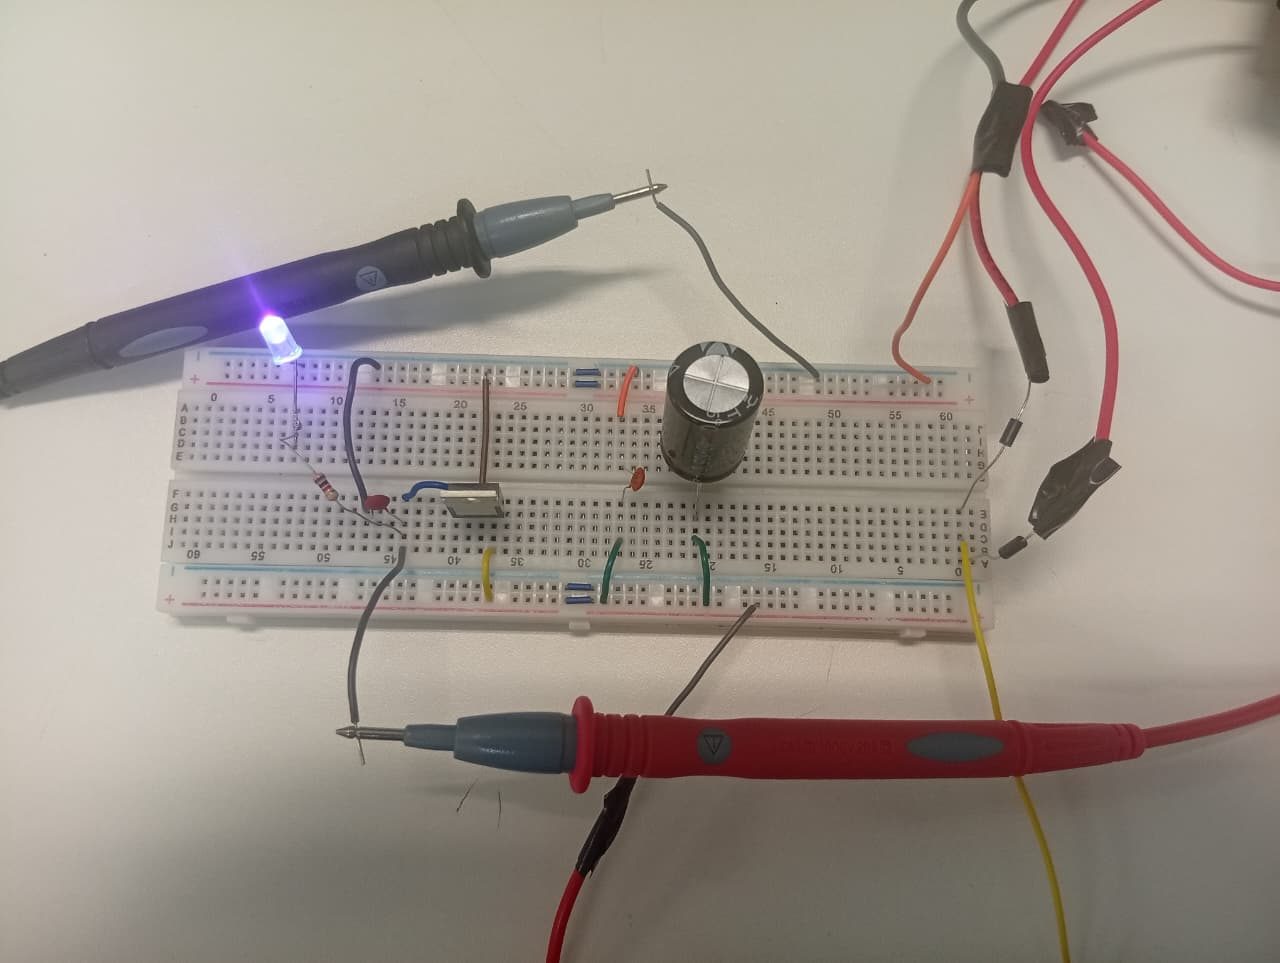
\includegraphics[width=\columnwidth,height=5.6cm,keepaspectratio]{Images/exp5_protoboard-multimetro_com-led.jpeg}
%\caption{Experimento 5 (etapa B) --- Montagem com carga (LED + resistor de $1\,\text{k}\Omega$) conectada.}
%\label{fig:exp5-com-led-proto}
%\end{figure}

\begin{figure}[H]
\centering
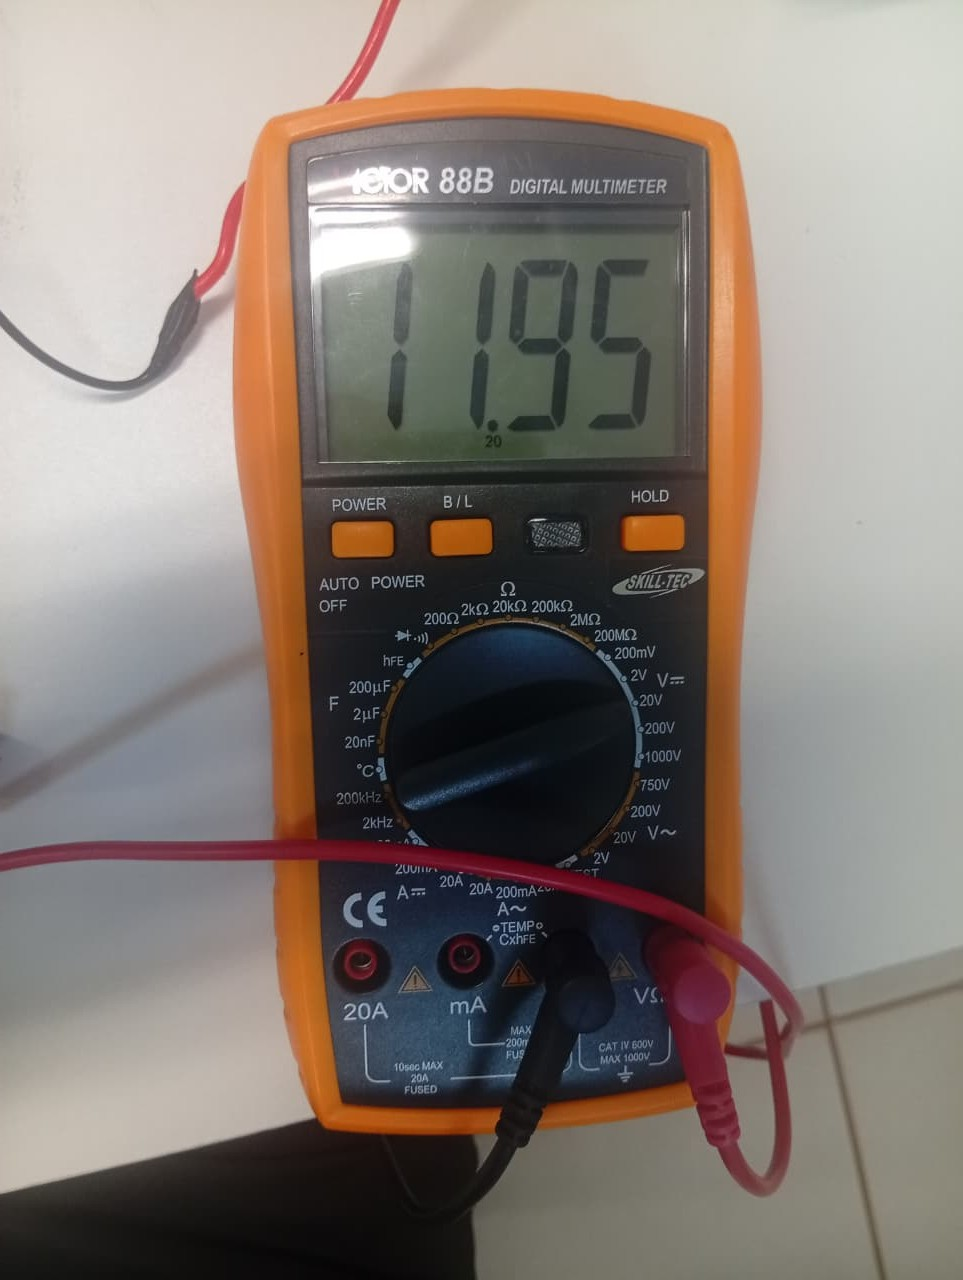
\includegraphics[width=\columnwidth,height=5.6cm,keepaspectratio]{Images/exp5_multimetro_com-led.jpeg}
\caption{Experimento 5 --- Multímetro Victor 88B na escala $20\,\text{V}$ DC indicando $11{,}95\,\text{V}$ com LED + $1\,\text{k}\Omega$.}
\label{fig:exp5-com-led-multi}
\end{figure}

\textbf{Valores medidos.} Sem carga, a leitura foi $11{,}93\,\text{V}$ (Figura~\ref{fig:exp5-sem-led-multi}); com LED + $1\,\text{k}\Omega$, $11{,}95\,\text{V}$ (Figura~\ref{fig:exp5-com-led-multi}), igual à leitura do Experimento~4 na mesma condição. A diferença é $+0{,}02\,\text{V}$.

\textbf{Incerteza e interpretação.} A incerteza adotada para o multímetro na escala de $20\,\text{V}$ DC, $\pm(0{,}5\% + 2\ \text{dígitos})$, resulta em $\pm(0{,}5\% \times 11{,}95 + 0{,}02) \approx \pm 0{,}08\,\text{V}$. As duas leituras são, portanto, indistinguíveis. A tensão não diminuiu com a carga, que seria o sentido esperado, mas aumentou $0{,}02\,\text{V}$, valor inferior à incerteza. A regulação de carga, definida como $(V_{\text{sem}} - V_{\text{com}})/V_{\text{com}}$, é
\begin{equation}
\frac{11{,}93 - 11{,}95}{11{,}95} \approx -0{,}17\%,
\end{equation}
valor menor que a incerteza relativa de $\approx 0{,}67\%$ e sem significado físico próprio. A variação de corrente entre as duas condições, $\Delta I \approx 9\,\text{mA}$ (cálculo com $V_F \approx 3{,}0\,\text{V}$, hipótese, não verificada), não exercita a regulação do LM7812. A tensão sob a carga de $100\,\Omega$ não foi registrada; o valor de $11{,}95\,\text{V}$ usado no Experimento~6 corresponde à condição com LED + $1\,\text{k}\Omega$. Este experimento não tem poder discriminativo para a regulação de carga.

\subsection{Experimento 6 --- Teste de Corrente com Carga de $100\,\Omega$}

\textbf{Condição.} O multímetro foi inserido em série entre o pino~3 do LM7812 e um resistor de $100\,\Omega \pm 5\%$ ligado ao GND, com a ponta vermelha no borne de $20\,\text{A}$ e a ponta preta no borne COM (Figuras~\ref{fig:exp6-proto} e~\ref{fig:exp6-corrente}).

\begin{figure}[H]
\centering
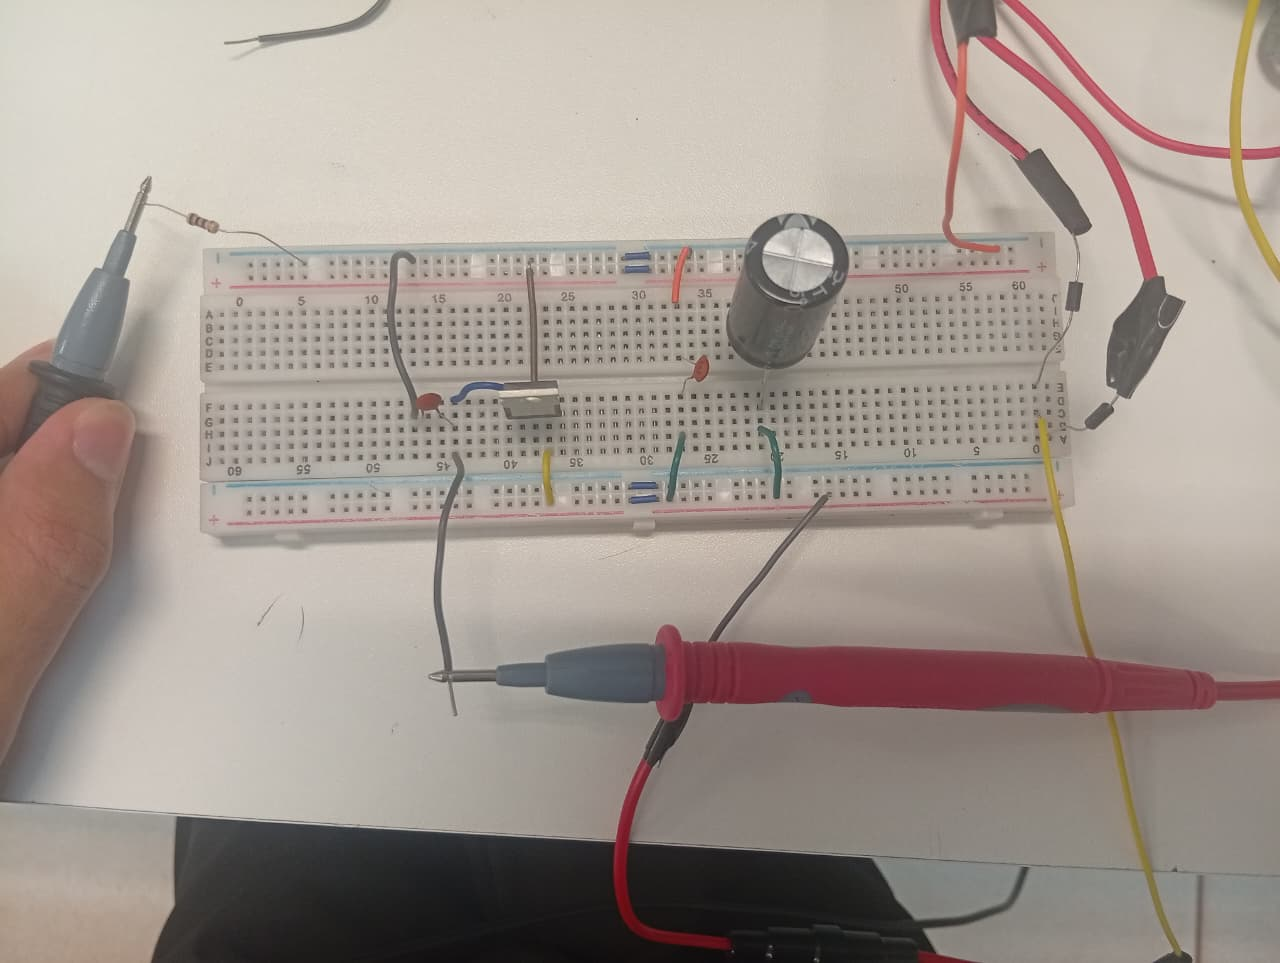
\includegraphics[width=\columnwidth,height=5.6cm,keepaspectratio]{Images/exp6_protoboard-multimetro_com-resistencia-100-ohm-corrente.jpeg}
\caption{Experimento 6 --- Montagem com o multímetro em série entre o pino~3 do LM7812 e o resistor de $100\,\Omega$ ao GND.}
\label{fig:exp6-proto}
\end{figure}

\begin{figure}[H]
\centering
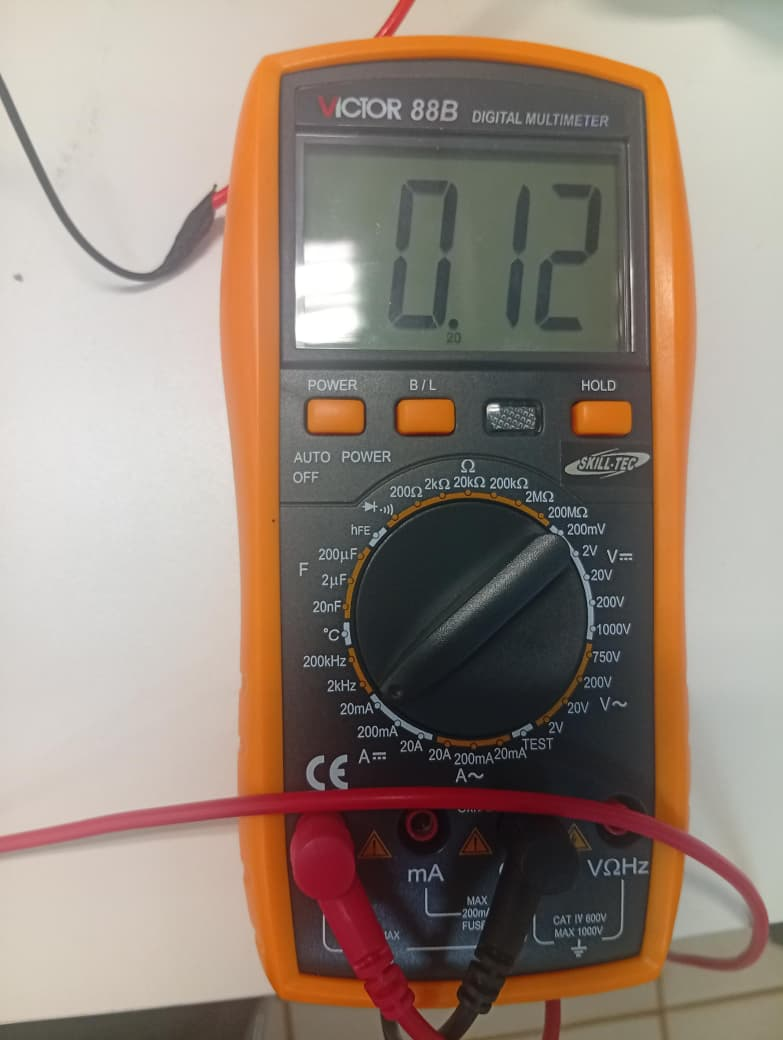
\includegraphics[width=\columnwidth,height=5.6cm,keepaspectratio]{Images/exp6_multimetro_com-resistencia-100-ohm-corrente.jpeg}
\caption{Experimento 6 --- Multímetro Victor 88B com ponta vermelha no borne $20\,\text{A}$, indicando $0{,}12\,\text{A}$ ($120\,\text{mA}$) DC sobre a carga de $100\,\Omega$. A posição do seletor na fotografia não coincide com o borne utilizado.}
\label{fig:exp6-corrente}
\end{figure}

\textbf{Valor medido.} O visor (Figura~\ref{fig:exp6-corrente}) indica $0{,}12\,\text{A}$, com resolução de $0{,}01\,\text{A}$. A posição do seletor na fotografia não coincide com o borne de $20\,\text{A}$ utilizado; a leitura é registrada como indicada.

\textbf{Esperado e desvio.} Com $V_o = 11{,}95\,\text{V}$ (medido com LED + $1\,\text{k}\Omega$):
\begin{equation}
I_{\text{teór}} = \frac{V_o}{R} = \frac{11{,}95\,\text{V}}{100\,\Omega} = 0{,}1195\,\text{A} = 119{,}5\,\text{mA}.
\label{eq:ohm}
\end{equation}
Com a tolerância de $\pm 5\%$ do resistor, a faixa esperada é $11{,}95/105 \approx 113{,}8\,\text{mA}$ a $11{,}95/95 \approx 125{,}8\,\text{mA}$. A leitura de $0{,}12\,\text{A}$ (desvio de $+0{,}4\%$ em relação a $119{,}5\,\text{mA}$), com resolução de $0{,}01\,\text{A}$, é compatível com essa faixa. A queda de tensão do amperímetro e o valor real do resistor não foram avaliados.

\textbf{Potência no resistor.} A potência dissipada é $P = V_o I = 11{,}95 \times 0{,}1195 \approx 1{,}43\,\text{W}$. Um resistor de $1/4\,\text{W}$ ficaria sobrecarregado ($\approx 5{,}7$ vezes sua potência nominal). A potência nominal do resistor utilizado não foi registrada. Recomenda-se resistor de potência nominal $\geq 2\,\text{W}$ para esse ensaio.

\subsection{Verificação Teórica a $1\,\text{A}$ (Análise Teórica, Não Ensaiada)}
\label{sec:teoria1A}

Esta subseção é uma análise teórica, não ensaiada: a fonte foi validada experimentalmente até $0{,}12\,\text{A}$ e projetada e analisada para $1\,\text{A}$. As premissas são: secundário de $12\,\text{V}$ RMS a $1\,\text{A}$ (especificação do trabalho; a tensão sob carga não foi medida), $V_D = 0{,}7\,\text{V}$, $f_{\text{ret}} = 120\,\text{Hz}$, $C = 4700\,\mu\text{F}$ e entrada mínima do regulador de $12\,\text{V} + 2\,\text{V} = 14\,\text{V}$ (\textit{dropout} de \textit{datasheet}~\cite{ds_lm7812}).

\textbf{Rede nominal.}
\begin{equation}
V_{p,\text{ret}} = 12\sqrt{2} - 0{,}7 \approx 16{,}27\,\text{V},
\label{eq:teoria_nom}
\end{equation}
\begin{equation}
\Delta V_r = \frac{1\,\text{A}}{120 \times 4700\,\mu\text{F}} \approx 1{,}77\,\text{V}_{\text{pp}},
\label{eq:teoria_ripple}
\end{equation}
\begin{equation}
V_{\text{vale}} = 16{,}27 - 1{,}77 \approx 14{,}5\,\text{V}.
\label{eq:teoria_vale}
\end{equation}
Em relação ao mínimo de $\approx 14\,\text{V}$, a margem é de $\approx 0{,}5\,\text{V}$.

\textbf{Rede $-10\%$.} Com $0{,}9 \times 12\,\text{V}$:
\begin{equation}
V_{p,\text{ret}} = 0{,}9 \times 12\sqrt{2} - 0{,}7 \approx 14{,}57\,\text{V},
\label{eq:teoria_rede}
\end{equation}
\begin{equation}
V_{\text{vale}} = 14{,}57 - 1{,}77 \approx 12{,}8\,\text{V}.
\end{equation}
Como $12{,}8\,\text{V} < 14\,\text{V}$, o regulador sai de regulação nos vales e o \textit{ripple} aparece na saída.

\textbf{Dissipação no regulador.} A tensão média na entrada é $V_{\text{méd}} \approx 16{,}27 - 1{,}77/2 \approx 15{,}4\,\text{V}$, e
\begin{equation}
P_D \approx (15{,}4 - 12) \times 1\,\text{A} \approx 3{,}4\,\text{W}.
\label{eq:teoria_pd}
\end{equation}
O valor de $6{,}0\,\text{W}$, obtido com a tensão sem carga, $(17{,}96 - 11{,}95) \times 1\,\text{A}$, é apenas um limite superior.

\textbf{Análise térmica.} Adota-se $T_a = 30\,^\circ\mathrm{C}$ (hipótese, não verificada). Como o componente utilizado possui gravação comercial SCE7812, sem folha de dados própria publicada pelo fabricante ou distribuidor, adotam-se os parâmetros térmicos do \href{https://www.ti.com/lit/ds/symlink/lm340.pdf}{Datasheet do LM7812}. Conforme os valores clássicos apresentados na seção 6.1 do documento, utilizam-se $R_{\theta JA} = 54\,^\circ\mathrm{C/W}$ e $R_{\theta JC} = 4\,^\circ\mathrm{C/W}$, além de $T_{j,\max} = 150\,^\circ\mathrm{C}$ (máximo absoluto, com operação recomendada até $125\,^\circ\mathrm{C}$). Sem dissipador,

\begin{equation}
\Delta T = P_D R_{\theta JA} \approx 3{,}4\,\mathrm{W} \times 54\,^\circ\mathrm{C/W} = 183{,}6\,^\circ\mathrm{C},
\tag{19}
\end{equation}

\begin{equation}
T_j = T_a + \Delta T = 30 + 183{,}6 = 213{,}6\,^\circ\mathrm{C},
\tag{20}
\end{equation}

e verifica-se que $T_j > T_{j,\max}$, indicando que a operação sem dissipador não é termicamente adequada. O dissipador necessário deve satisfazer

\begin{equation}
R_{\theta SA} \leq \frac{T_{j,\max} - T_a}{P_D} - R_{\theta JC} - R_{\theta CS},
\tag{21}
\end{equation}

com $R_{\theta CS}$ representando a resistência térmica da interface caixa--dissipador. Como não foi utilizado dissipador, esse parâmetro não se aplica à montagem realizada. O dissipador não consta na Tabela I, pois não foi adquirido.

\subsection{Síntese dos Resultados Experimentais}

A Tabela~\ref{tab:resumo} consolida os valores esperados ou calculados e as grandezas medidas.

\begin{table*}[t]
\renewcommand{\tablename}{TABELA}
\caption{Resumo comparativo entre valores esperados/calculados e medições.}
\label{tab:resumo}
\centering
\scriptsize
\setlength{\tabcolsep}{4pt}
\begin{tabular}{lp{2.4cm}p{3.1cm}p{3.3cm}p{1.5cm}p{4.9cm}}
\hline
Exp. & Condição & Esperado/calculado & Medido & Desvio (\%) & Observação \\
\hline
1 & Secundário em vazio (osciloscópio) & $60\,\text{Hz}$; $V_{\text{RMS}}$ nominal $12\,\text{V}$ & $60{,}01\,\text{Hz}$ (contador); $V_{p} = 19{,}1\,\text{V}$ (exibido $V_{\text{pp}} = 382\,\text{V}$, fator $1/10$); $V_{\text{RMS}} \approx 13{,}5\,\text{V}$ & $+0{,}01$ (freq.); $+12{,}5$ ($V_{\text{RMS}}$) & Atenuação $10\times$ (fator $1/10$) validada; $59{,}8\,\text{Hz}$ no osciloscópio ($-0{,}33\%$). \\
1 & Secundário em vazio (multímetro) & $V_{\text{RMS}} \approx 13{,}5\,\text{V}$ (osciloscópio), função V$\sim$ & $0{,}00\,\text{V}$ (função DC) & -- & Falha de procedimento; não é resultado do ensaio. \\
2A & Pós-diodos, $1\,\text{k}\Omega$, sem filtro & $V_{\text{DC}} = 12{,}16\,\text{V}$ ($V_p = 19{,}1\,\text{V}$); $11{,}71\,\text{V}$ ($18{,}4\,\text{V}$) & $\text{Mean} = 11{,}9\,\text{V}$; $120{,}08\,\text{Hz}$ (contador) & $-2{,}1$; $+1{,}6$ & Concordância dentro de $\approx \pm 2\%$; fator $1\times$; $V_{\text{pp}} = 19{,}1\,\text{V}$, $T = 8{,}36\,\text{ms}$. \\
2B & Com $4700\,\mu\text{F}$ & Nível DC próximo ao pico ($18{,}4\,\text{V}$) & $17{,}9\,\text{V}$ (exibido $179\,\text{V}$, fator $1/10$); $17{,}96\,\text{V}$ (multímetro, Exp.~3) & $-2{,}7$ & Resultado válido: nível DC. Janela de $240\,\mu\text{s}$ não mostra o \textit{ripple}. \\
3A & Pino 1, DC & $\geq 14\,\text{V}$ ($12\,\text{V}$ + \textit{dropout}) & $17{,}96\,\text{V}$ & -- & Validado; margem $\approx 4\,\text{V}$ sobre $14\,\text{V}$ e $\approx 6\,\text{V}$ sobre $12\,\text{V}$. \\
3B/C & \textit{Ripple} no pino 1, sem $\to$ com LED & $8{,}9 \to 24{,}8\,\text{mV}_{\text{pp}}$ & $\approx 1{,}3 \to 3{,}0\,\text{mV}_{\text{pp}}$ (exibidos) & $-85$; $-88$ & Amplitude absoluta não validada (fator da ponta não registrado); crescimento de $2{,}3\times$ contra $2{,}8\times$ previsto. \\
4 & Pino 3 com LED + $1\,\text{k}\Omega$, DC & $12{,}00\,\text{V}$ ($11{,}5$ a $12{,}5\,\text{V}$) & $11{,}95\,\text{V}$ & $-0{,}42$ & Dentro de $\pm 4\%$. \\
4 & \textit{Ripple} no pino 3 & Muito menor que na entrada & $\lesssim 0{,}6\,\text{mV}_{\text{pp}}$ (limite de leitura) & -- & Redução $\approx 14$ a $16\,\text{dB}$, apenas limite inferior; $55$ a $70\,\text{dB}$ são de \textit{datasheet}, não medidos. \\
5 & Sem $\times$ com LED + $1\,\text{k}\Omega$ & Sem variação detectável ($<$ incerteza de $\pm 0{,}08\,\text{V}$) & $11{,}93\,\text{V}$ e $11{,}95\,\text{V}$ & $-0{,}17$ (regulação de carga) & Leituras indistinguíveis; $\Delta I \approx 9\,\text{mA}$ não exercita a regulação. \\
6 & Carga de $100\,\Omega$, amperímetro em série & $119{,}5\,\text{mA}$ ($113{,}8$ a $125{,}8\,\text{mA}$) & $0{,}12\,\text{A}$ & $+0{,}4$ & Compatível; resolução de $0{,}01\,\text{A}$; $P = 1{,}43\,\text{W}$ no resistor. \\
\hline
\end{tabular}
\end{table*}



\FloatBarrier
\section{Conclusão}

Foram montadas e ensaiadas em \textit{protoboard} as etapas de uma fonte linear regulada de $12\,\text{V}$ DC (transformador de $12\,\text{V}+12\,\text{V}$, retificador de onda completa, filtro capacitivo de $4700\,\mu\text{F}$ e regulador LM7812). Os objetivos do trabalho foram cumpridos dentro dos limites descritos a seguir.

Os resultados validados são: tensão filtrada de $17{,}96\,\text{V}$ no pino~1 do regulador, com \textit{ripple} em dente de serra de $120\,\text{Hz}$ que cresce com a carga; saída de $11{,}95\,\text{V}$, desvio de $-0{,}42\%$ em relação a $12\,\text{V}$ e dentro da faixa de $\pm 4\%$ do \textit{datasheet}; \textit{ripple} de saída abaixo do limite de leitura, sem o dente de serra visto na entrada; e corrente de $0{,}12\,\text{A}$ sobre o resistor de $100\,\Omega$, compatível com a lei de Ohm dentro da tolerância do resistor.

As limitações são: a corrente máxima ensaiada foi de $0{,}12\,\text{A}$, e a operação em $1\,\text{A}$ foi apenas analisada teoricamente; a atenuação configurada no osciloscópio foi inconsistente entre as capturas, e a amplitude absoluta do \textit{ripple} não está validada; o multímetro foi utilizado na função DC no Experimento~1; e o Experimento~5 não tem poder discriminativo para a regulação de carga.

Como melhorias, recomendam-se dissipador no regulador, fusível de retardo de $250\,\text{V}$ CA, resistor de potência nominal $\geq 2\,\text{W}$ para o ensaio de corrente, ensaio a $1\,\text{A}$, transferência para placa de circuito impresso em caixa e medição do \textit{ripple} com ponta e canal padronizados e sem filtros.


\section*{Referências}

\begin{thebibliography}{00}

% Roteiro do experimento
\bibitem{roteiro} D. L. Catelan, {\it Trabalho: Fonte 12V e 1A.} Roteiro do Trabalho (Disciplina de Circuitos Eletrônicos), Faculdade de Computação, Universidade Federal de Mato Grosso do Sul (UFMS), Campo Grande, MS. [Online]. Disponível em: \url{https://ava.ufms.br/pluginfile.php/2836122/mod_resource/content/0/Trabalho%20Pr%C3%A1tico%20-%20Fonte%20de%20alimenta%C3%A7%C3%A3o.pdf}.

% Livro do boylestad
\bibitem{boylestad} R. L. Boylestad e L. Nashelsky, {\it Dispositivos Eletrônicos e Teoria de Circuitos,} 11$^{\mathrm{a}}$ ed. São Paulo, SP, Brasil: Pearson, 2013.

% 3. Livro clássico de laboratório (citado no roteiro)
\bibitem{capuano} F. G. Capuano e M. A. M. Marino, {\it Laboratório de Eletricidade e Eletrônica,} 24$^{\mathrm{a}}$ ed. São Paulo, SP, Brasil: Editora Érica, 2010.

% 4. Outro livro clássico de eletrônica (citado no roteiro)
\bibitem{sedra} A. S. Sedra e K. C. Smith, {\it Microeletrônica,} 5$^{\mathrm{a}}$ ed. São Paulo, SP, Brasil: Pearson Prentice Hall, 2007.

% 5. Falstad
\bibitem{falstad} P. Falstad, ``Circuit Simulator Applet'', {\it Falstad.com}. [Online]. Disponível em: \url{http://www.falstad.com/circuit/}. Acesso em: ago. 2026.

% 6. Datasheet do regulador LM7812 (LM340)
\bibitem{ds_lm7812} Texas Instruments, {\it LM340, LM340A and LM7805 Family Wide VIN 1.5-A Fixed Voltage Regulators,} Datasheet SNOSBT0L. [Online]. Disponível em: \url{https://www.ti.com/lit/ds/symlink/lm340.pdf}.

% 7. Datasheet do diodo 1N4007
\bibitem{ds_1n4007} Vishay Semiconductors, {\it 1N4001 through 1N4007 General Purpose Plastic Rectifier,} Datasheet. [Online]. Disponível em: \url{https://www.vishay.com/docs/88503/1n4001.pdf}.

\end{thebibliography}


\end{document}
